\documentclass[12pt,a4paper]{article}

% Packages
\usepackage[utf8]{inputenc}
\usepackage[T1]{fontenc}
\usepackage{lmodern} % Latin Modern fonts
\usepackage{amsmath,amssymb,amsthm}
\usepackage{geometry}
\usepackage{graphicx}
\usepackage{xcolor}
\usepackage{listings}
\usepackage{float}
\usepackage{booktabs}
\usepackage{longtable}
\usepackage{array}
\usepackage{fancyhdr}
\usepackage{hyperref}
\usepackage{enumitem}
\usepackage{mdframed}
\usepackage{parskip}
\usepackage{setspace}
\usepackage{titlesec}
\usepackage{multirow}
\usepackage{tikz}
\usetikzlibrary{shapes,arrows,positioning,calc,shadows,fit,backgrounds}
\usepackage{pgfplots}
\pgfplotsset{compat=1.17}
\usepackage{smartdiagram}
\usepackage{flowchart}
\usepackage{chronology}

% Page setup
\geometry{margin=1in}
\pagestyle{fancy}
\fancyhf{}
\fancyhead[L]{\leftmark}
\fancyhead[R]{\thepage}
\setlength{\headheight}{14.5pt}
\setlength{\emergencystretch}{3em}
\sloppy
\hfuzz=30pt
\hbadness=10000

% Font settings
\renewcommand{\familydefault}{\sfdefault} % Sans serif as default
\titleformat{\section}{\Large\bfseries\sffamily}{\thesection}{1em}{}
\titleformat{\subsection}{\large\bfseries\sffamily}{\thesubsection}{1em}{}
\titleformat{\subsubsection}{\normalsize\bfseries\sffamily}{\thesubsubsection}{1em}{}

% Code listing settings
\lstset{
    basicstyle=\ttfamily\footnotesize,
    keywordstyle=\color{blue}\bfseries,
    commentstyle=\color{gray}\itshape,
    stringstyle=\color{red},
    numbers=left,
    numberstyle=\tiny,
    frame=single,
    breaklines=true,
    captionpos=b,
    showstringspaces=false
}

% Colors
\definecolor{codebg}{rgb}{0.95,0.95,0.95}
\definecolor{accent}{rgb}{0.2,0.6,0.8}
\definecolor{success}{rgb}{0.2,0.8,0.2}
\definecolor{warning}{rgb}{0.9,0.6,0.1}

% Custom commands
\newcommand{\code}[1]{\texttt{#1}}
\newcommand{\highlight}[1]{\colorbox{yellow}{#1}}
\newcommand{\important}[1]{\mdframed[backgroundcolor=blue!10,linecolor=blue!50]{\textbf{Important:} #1}}

% Title
\title{\Huge\sffamily\textbf{NurseNotes Clone}\\[\baselineskip]
\large\textit{AI-Powered Lecture Intelligence Platform for Nursing Students}\\[2\baselineskip]
\large Comprehensive Development Guide}

\author{\sffamily Manu Vashistha}
\date{\today}

\begin{document}

\maketitle
\tableofcontents
\newpage

\section{Project Overview}

\subsection{Application Description}

NurseNotes Clone is a sophisticated web application designed to revolutionize how nursing students interact with educational content. The platform leverages artificial intelligence to transform lecture recordings into structured, actionable learning materials.

\subsubsection{Core Features}
\begin{itemize}
    \item \textbf{Audio/Video Upload}: Support for multiple lecture recording formats
    \item \textbf{AI-Powered Transcription}: AssemblyAI integration for accurate speech-to-text conversion
    \item \textbf{Intelligent Analysis}: Multi-modal AI processing using Google Gemini, Mistral AI, and OpenAI
    \item \textbf{Structured Output}: Automated generation of summaries, clinical concepts, and study guides
    \item \textbf{User Authentication}: Secure Auth0-based login system
    \item \textbf{Actionable Insights}: Email and WhatsApp integration for sharing learning materials
    \item \textbf{Modern UI/UX}: Responsive design with Tailwind CSS and React components
\end{itemize}

\subsection{Technology Stack}

\begin{table}[H]
\centering
\caption{Technology Stack Overview}
\label{tab:tech-stack}
\begin{tabular}{@{}lll@{}}
\toprule
\textbf{Category} & \textbf{Technology} & \textbf{Purpose} \\
\midrule
Frontend & React 18 & UI Framework \\
& Next.js 14 & Full-Stack Framework \\
& TypeScript & Type Safety \\
& Tailwind CSS & Styling Framework \\
& Lucide React & Icon Library \\
\midrule
Backend & Next.js API Routes & Server-Side Logic \\
& Node.js 20 & Runtime Environment \\
& PostgreSQL & Database \\
& Auth0 & Authentication \\
\midrule
AI/ML & Google Gemini AI & Content Analysis \\
& Mistral AI & Text Processing \\
& OpenAI GPT & Advanced Reasoning \\
& AssemblyAI & Audio Transcription \\
\midrule
Media Processing & FFmpeg & Video/Audio Processing \\
& Fluent-FFmpeg & Node.js FFmpeg Wrapper \\
\midrule
Communication & Twilio & SMS/WhatsApp Integration \\
& Nodemailer & Email Services \\
\midrule
Deployment & Docker & Containerization \\
& Render & Cloud Platform \\
& GitHub Actions & CI/CD \\
\bottomrule
\end{tabular}
\end{table}

\section{Architecture and Design}

\subsection{System Architecture}

\subsubsection{System Architecture Overview}

The NurseNotes Clone application follows a modern web architecture with clear separation of concerns:

\begin{figure}[H]
\centering
\resizebox{0.9\textwidth}{!}{%
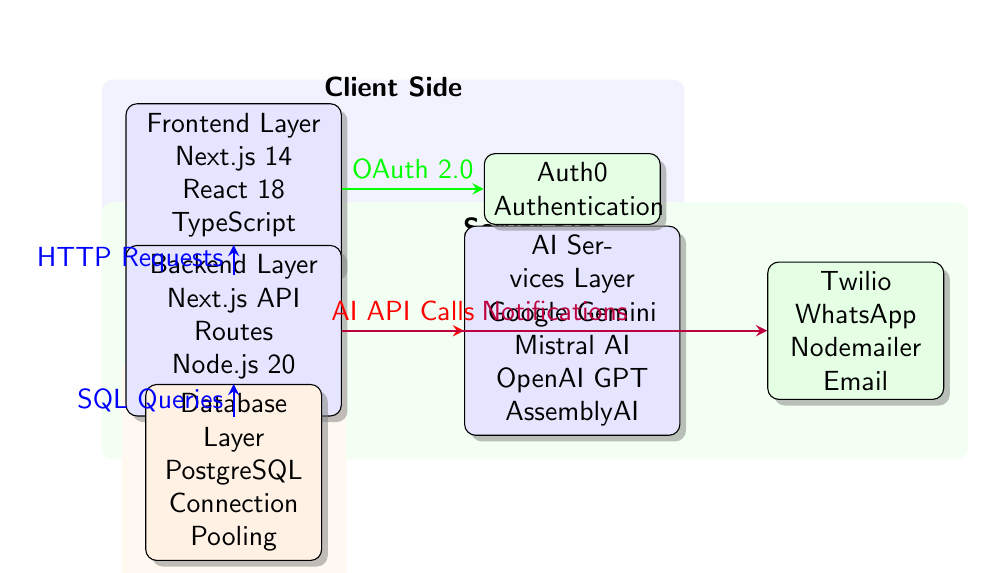
\begin{tikzpicture}[
    node distance=1.8cm,
    box/.style={rectangle, draw=black, fill=blue!10, text width=2.5cm, text centered, rounded corners, minimum height=1.2cm, drop shadow},
    service/.style={rectangle, draw=black, fill=green!10, text width=2cm, text centered, rounded corners, minimum height=0.8cm, drop shadow},
    database/.style={rectangle, draw=black, fill=orange!10, text width=2cm, text centered, rounded corners, minimum height=0.8cm, drop shadow},
    arrow/.style={->,>=stealth,thick}
]

% Frontend Layer
\node[box] (frontend) {Frontend Layer\\Next.js 14\\React 18\\TypeScript\\Tailwind CSS};

% Backend Layer
\node[box, below of=frontend] (backend) {Backend Layer\\Next.js API Routes\\Node.js 20\\RESTful API};

% Database Layer
\node[database, below of=backend] (database) {Database Layer\\PostgreSQL\\Connection Pooling};

% AI Services Layer
\node[box, right of=backend, xshift=2.5cm] (ai) {AI Services Layer\\Google Gemini\\Mistral AI\\OpenAI GPT\\AssemblyAI};

% External Services
\node[service, right of=frontend, xshift=2.5cm] (auth) {Auth0\\Authentication};

\node[service, right of=ai, xshift=1.8cm] (comm) {Twilio\\WhatsApp\\Nodemailer\\Email};

% Connections
\draw[arrow, blue] (frontend) -- (backend) node[midway,left] {HTTP Requests};
\draw[arrow, blue] (backend) -- (database) node[midway,left] {SQL Queries};
\draw[arrow, red] (backend) -- (ai) node[midway,above] {AI API Calls};
\draw[arrow, green] (frontend) -- (auth) node[midway,above] {OAuth 2.0};
\draw[arrow, purple] (backend) -- (comm) node[midway,above] {Notifications};

% Background layers
\begin{scope}[on background layer]
    \node[fit=(frontend)(auth), fill=blue!5, rounded corners, inner sep=0.3cm] (client) {};
    \node[above of=client, yshift=-0.5cm] {\textbf{Client Side}};
    
    \node[fit=(backend)(ai)(comm), fill=green!5, rounded corners, inner sep=0.3cm] (server) {};
    \node[above of=server, yshift=-0.5cm] {\textbf{Server Side}};
    
    \node[fit=(database), fill=orange!5, rounded corners, inner sep=0.3cm] (data) {};
    \node[above of=data, yshift=-0.5cm] {\textbf{Data Layer}};
\end{scope}

\end{tikzpicture}
}
\caption{Complete System Architecture Diagram}
\label{fig:system-architecture}
\end{figure}

\clearpage

\subsubsection{Detailed Component Architecture}

\begin{figure}[H]
\centering
\resizebox{0.85\textwidth}{!}{%
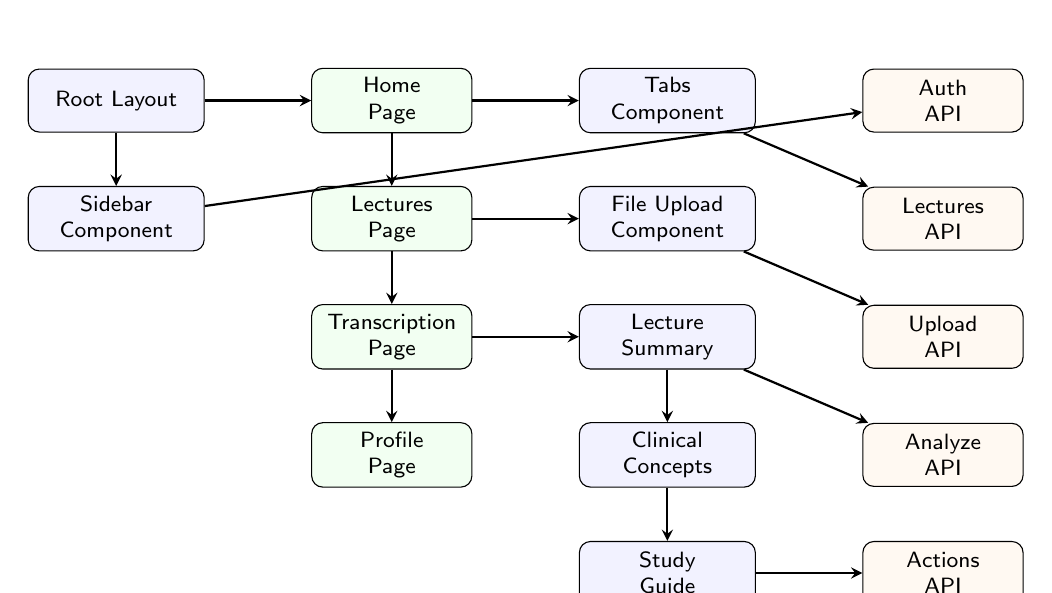
\begin{tikzpicture}[
    node distance=1.5cm,
    component/.style={rectangle, draw=black, fill=blue!5, text width=2cm, text centered, rounded corners, minimum height=0.8cm, font=\footnotesize},
    page/.style={rectangle, draw=black, fill=green!5, text width=1.8cm, text centered, rounded corners, minimum height=0.8cm, font=\footnotesize},
    api/.style={rectangle, draw=black, fill=orange!5, text width=1.8cm, text centered, rounded corners, minimum height=0.8cm, font=\footnotesize},
    arrow/.style={->,>=stealth,thick}
]

% Layout Components
\node[component] (layout) {Root Layout};
\node[component, below of=layout] (sidebar) {Sidebar\\Component};

% Page Components
\node[page, right of=layout, xshift=2cm] (home) {Home\\Page};
\node[page, below of=home] (lectures) {Lectures\\Page};
\node[page, below of=lectures] (transcription) {Transcription\\Page};
\node[page, below of=transcription] (profile) {Profile\\Page};

% Feature Components
\node[component, right of=home, xshift=2cm] (tabs) {Tabs\\Component};
\node[component, below of=tabs] (upload) {File Upload\\Component};
\node[component, below of=upload] (summary) {Lecture\\Summary};
\node[component, below of=summary] (concepts) {Clinical\\Concepts};
\node[component, below of=concepts] (studyguide) {Study\\Guide};

% API Components
\node[api, right of=tabs, xshift=2cm] (authapi) {Auth\\API};
\node[api, below of=authapi] (lecturesapi) {Lectures\\API};
\node[api, below of=lecturesapi] (uploadapi) {Upload\\API};
\node[api, below of=uploadapi] (analyzeapi) {Analyze\\API};
\node[api, below of=analyzeapi] (actionsapi) {Actions\\API};

% Connections
\draw[arrow] (layout) -- (sidebar);
\draw[arrow] (layout) -- (home);
\draw[arrow] (home) -- (lectures);
\draw[arrow] (lectures) -- (transcription);
\draw[arrow] (transcription) -- (profile);

\draw[arrow] (home) -- (tabs);
\draw[arrow] (lectures) -- (upload);
\draw[arrow] (transcription) -- (summary);
\draw[arrow] (summary) -- (concepts);
\draw[arrow] (concepts) -- (studyguide);

\draw[arrow] (sidebar) -- (authapi);
\draw[arrow] (tabs) -- (lecturesapi);
\draw[arrow] (upload) -- (uploadapi);
\draw[arrow] (summary) -- (analyzeapi);
\draw[arrow] (studyguide) -- (actionsapi);

\end{tikzpicture}
}
\caption{Detailed Component Architecture with Dependencies}
\label{fig:component-architecture}
\end{figure}

\clearpage

\subsubsection{Data Flow Architecture}

\begin{figure}[H]
\centering
\resizebox{0.95\textwidth}{!}{%
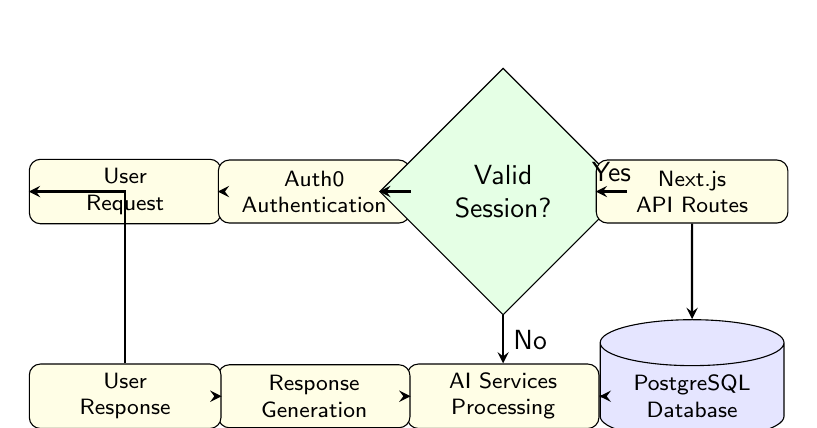
\begin{tikzpicture}[
    node distance=2.2cm,
    process/.style={rectangle, draw=black, fill=yellow!10, text width=2.2cm, text centered, rounded corners, minimum height=0.8cm, font=\footnotesize},
    data/.style={cylinder, draw=black, fill=blue!10, text width=2.1cm, text centered, minimum height=0.8cm, shape border rotate=90, aspect=0.25, font=\footnotesize},
    decision/.style={diamond, draw=black, fill=green!10, text width=2cm, text centered, minimum height=0.8cm},
    arrow/.style={->,>=stealth,thick}
]

\node[process] (user) {User\\Request};
\node[process, right of=user, xshift=0.2cm] (auth) {Auth0\\Authentication};
\node[decision, right of=auth, xshift=0.2cm] (authcheck) {Valid\\Session?};
\node[process, right of=authcheck, xshift=0.2cm] (api) {Next.js\\API Routes};
\node[data, below of=api, yshift=-0.4cm] (db) {PostgreSQL\\Database};
\node[process, below of=authcheck, yshift=-0.4cm] (ai) {AI Services\\Processing};
\node[process, left of=ai, xshift=-0.2cm] (response) {Response\\Generation};
\node[process, left of=response, xshift=-0.2cm] (userresp) {User\\Response};

\draw[arrow] (user) -- (auth);
\draw[arrow] (auth) -- (authcheck);
\draw[arrow] (authcheck) -- node[above] {Yes} (api);
\draw[arrow] (authcheck) -- node[right] {No} (ai);
\draw[arrow] (api) -- (db);
\draw[arrow] (db.west) -- (ai.east);
\draw[arrow] (ai) -- (response);
\draw[arrow] (response) -- (userresp);
\draw[arrow] (userresp.north) |- (user.west);

\end{tikzpicture}
}
\caption{Data Flow Architecture with Decision Points}
\label{fig:data-flow}
\end{figure}

\subsection{Component Architecture}

The application follows a modular component architecture with clear separation of concerns:

\subsubsection{Layout Components}
\begin{itemize}
    \item \textbf{Root Layout}: Main application layout with sidebar and main content area
    \item \textbf{Sidebar Component}: Navigation menu and user authentication status
    \item \textbf{Header Component}: Application branding and user information
\end{itemize}

\subsubsection{Page Components}
\begin{itemize}
    \item \textbf{Home Page}: Dashboard with overview and quick actions
    \item \textbf{Lectures Page}: List of uploaded lectures with management options
    \item \textbf{Transcription Page}: Analysis results with tabbed interface
    \item \textbf{Profile Page}: User profile and settings management
\end{itemize}

\subsubsection{Feature Components}
\begin{itemize}
    \item \textbf{File Upload Component}: Drag-and-drop file upload interface
    \item \textbf{Tabs Component}: Reusable tab interface for content organization
    \item \textbf{Lecture Summary Component}: Display of AI-generated summaries
    \item \textbf{Clinical Concepts Component}: Highlighted medical concepts
    \item \textbf{Study Guide Component}: Structured study materials
\end{itemize}

\subsubsection{API Components}
\begin{itemize}
    \item \textbf{Authentication API}: Auth0 integration and session management
    \item \textbf{Lectures API}: CRUD operations for lecture management
    \item \textbf{Upload API}: File handling and storage
    \item \textbf{Analysis API}: AI service integration and processing
    \item \textbf{Actions API}: Email and WhatsApp communication
\end{itemize}

\section{Database Design}

\subsection{Database Schema}

\subsubsection{Entity Relationship Diagram}

\begin{figure}[H]
\centering
\resizebox{0.9\textwidth}{!}{%
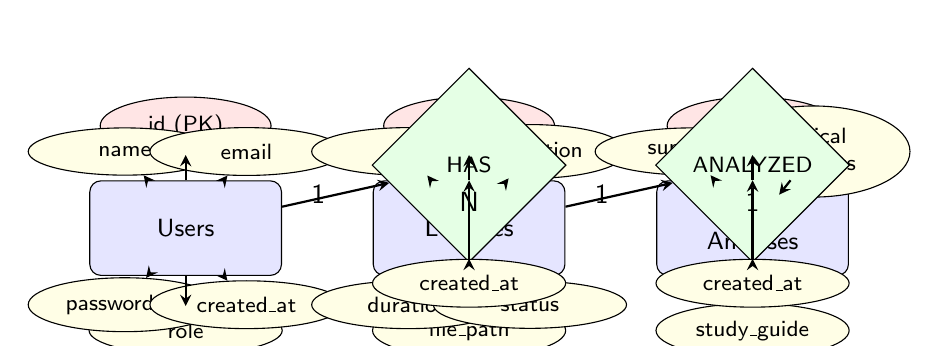
\begin{tikzpicture}[
    node distance=1.8cm,
    entity/.style={rectangle, draw=black, fill=blue!10, text width=2.2cm, text centered, rounded corners, minimum height=1.2cm, font=\small},
    attribute/.style={ellipse, draw=black, fill=yellow!10, text width=1.5cm, text centered, minimum height=0.6cm, font=\footnotesize},
    relationship/.style={diamond, draw=black, fill=green!10, text width=1.8cm, text centered, minimum height=0.8cm, font=\footnotesize},
    pk/.style={ellipse, draw=black, fill=red!10, text width=1.3cm, text centered, minimum height=0.6cm, font=\footnotesize},
    arrow/.style={->,>=stealth,thick}
]

% Entities
\node[entity] (users) {Users};
\node[entity, right of=users, xshift=1.8cm] (lectures) {Lectures};
\node[entity, right of=lectures, xshift=1.8cm] (analyses) {Lecture Analyses};

% Attributes for Users
\node[pk, above of=users, yshift=-0.5cm] (userid) {id (PK)};
\node[attribute, above left of=users, xshift=0.5cm, yshift=-0.3cm] (username) {name};
\node[attribute, above right of=users, xshift=-0.5cm, yshift=-0.3cm] (useremail) {email};
\node[attribute, below of=users, yshift=0.5cm] (userrole) {role};
\node[attribute, below left of=users, xshift=0.5cm, yshift=0.3cm] (userpass) {password\_hash};
\node[attribute, below right of=users, xshift=-0.5cm, yshift=0.3cm] (usercreated) {created\_at};

% Attributes for Lectures
\node[pk, above of=lectures, yshift=-0.5cm] (lectureid) {id (PK)};
\node[attribute, above left of=lectures, xshift=0.5cm, yshift=-0.3cm] (lecturetitle) {title};
\node[attribute, above right of=lectures, xshift=-0.5cm, yshift=-0.3cm] (lecturedesc) {description};
\node[attribute, below of=lectures, yshift=0.5cm] (lecturefile) {file\_path};
\node[attribute, below left of=lectures, xshift=0.5cm, yshift=0.3cm] (lectureduration) {duration};
\node[attribute, below right of=lectures, xshift=-0.5cm, yshift=0.3cm] (lecturestatus) {status};

% Attributes for Analyses
\node[pk, above of=analyses, yshift=-0.5cm] (analysisid) {id (PK)};
\node[attribute, above left of=analyses, xshift=0.5cm, yshift=-0.3cm] (analysissummary) {summary};
\node[attribute, above right of=analyses, xshift=-0.5cm, yshift=-0.3cm] (analysisconcepts) {clinical concepts};
\node[attribute, below of=analyses, yshift=0.5cm] (analysisstudy) {study\_guide};

% Relationships
\node[relationship, above of=lectures, yshift=-1cm] (has) {HAS};
\node[relationship, above of=analyses, yshift=-1cm] (analyzed) {ANALYZED};

% Connect entities to attributes
\draw[arrow] (users) -- (userid);
\draw[arrow] (users) -- (username);
\draw[arrow] (users) -- (useremail);
\draw[arrow] (users) -- (userrole);
\draw[arrow] (users) -- (userpass);
\draw[arrow] (users) -- (usercreated);

\draw[arrow] (lectures) -- (lectureid);
\draw[arrow] (lectures) -- (lecturetitle);
\draw[arrow] (lectures) -- (lecturedesc);
\draw[arrow] (lectures) -- (lecturefile);
\draw[arrow] (lectures) -- (lectureduration);
\draw[arrow] (lectures) -- (lecturestatus);

\draw[arrow] (analyses) -- (analysisid);
\draw[arrow] (analyses) -- (analysissummary);
\draw[arrow] (analyses) -- (analysisconcepts);
\draw[arrow] (analyses) -- (analysisstudy);

% Connect relationships
\draw[arrow] (users) -- (has) node[midway, left] {1};
\draw[arrow] (has) -- (lectures) node[midway, above] {N};
\draw[arrow] (lectures) -- (analyzed) node[midway, left] {1};
\draw[arrow] (analyzed) -- (analyses) node[midway, above] {1};

% Relationship attributes
\node[attribute, below of=has, yshift=0.3cm] (lecturecreated) {created\_at};
\node[attribute, below of=analyzed, yshift=0.3cm] (analysiscreated) {created\_at};

\draw[arrow] (has) -- (lecturecreated);
\draw[arrow] (analyzed) -- (analysiscreated);

\end{tikzpicture}
}
\caption{Complete Entity Relationship Diagram}
\label{fig:er-diagram}
\end{figure}

\subsubsection{Database Schema Tables}

The application uses PostgreSQL with the following core tables:

\begin{table}[H]
\centering
\caption{Database Schema}
\label{tab:database-schema}
\scriptsize
\begin{tabular}{@{}>{\raggedright\arraybackslash}p{2.2cm}>{\raggedright\arraybackslash}p{2.8cm}>{\raggedright\arraybackslash}p{2.5cm}>{\raggedright\arraybackslash}p{6.0cm}@{}}
\toprule
\textbf{Table} & \textbf{Column} & \textbf{Type} & \textbf{Description} \\
\midrule
\multirow{6}{*}{users} & id & VARCHAR(255) & Primary Key \\
& name & VARCHAR(255) & User full name \\
& email & VARCHAR(255) & Email address (unique) \\
& password\_hash & TEXT & Hashed password \\
& role & VARCHAR(50) & User role (student/teacher/admin) \\
& created\_at & TIMESTAMP & Creation timestamp \\
\midrule
\multirow{7}{*}{lectures} & id & VARCHAR(255) & Primary Key \\
& user\_id & VARCHAR(255) & Foreign Key to users \\
& title & VARCHAR(500) & Lecture title \\
& description & TEXT & Lecture description \\
& file\_path & VARCHAR(1000) & File storage path \\
& duration & INTEGER & Duration in seconds \\
& status & VARCHAR(50) & Processing status \\
& created\_at & TIMESTAMP & Creation timestamp \\
\midrule
\multirow{5}{*}{lecture\_analyses} & id & VARCHAR(255) & Primary Key \\
& lecture\_id & VARCHAR(255) & Foreign Key to lectures \\
& summary & TEXT & AI-generated summary \\
& clinical\_concepts & JSONB & Clinical concepts array \\
& study\_guide & TEXT & Study guide content \\
& created\_at & TIMESTAMP & Creation timestamp \\
\bottomrule
\end{tabular}
\normalsize
\end{table}

\subsection{Database Connection}

The application uses a connection pool for efficient database management:

\begin{lstlisting}[caption=Database Connection Setup]
import { Pool } from 'pg';

const pool = new Pool({
  connectionString: process.env.DATABASE_URL,
  ssl: process.env.NODE_ENV === 'production' ? { rejectUnauthorized: false } : false
});

export async function initDb() {
  // Initialize database connection
}

export async function db() {
  return pool;
}
\end{lstlisting}

\subsection{Database Relationships}

\subsubsection{User-Lectures Relationship}
Each user can have multiple lectures (one-to-many relationship). The \code{user\_id} foreign key in the lectures table establishes this relationship.

\subsubsection{Lecture-Analysis Relationship}
Each lecture has one analysis record (one-to-one relationship). The \code{lecture\_id} foreign key in the lecture\_analyses table links analysis results to specific lectures.

\subsubsection{Indexing Strategy}
\begin{itemize}
    \item \code{users.email}: Unique index for fast user lookup
    \item \code{lectures.user\_id}: Index for user-specific lecture queries
    \item \code{lectures.created\_at}: Index for chronological ordering
    \item \code{lecture\_analyses.lecture\_id}: Unique index for analysis lookup
\end{itemize}

\section{API Design}

\subsection{API Endpoints}

\begin{table}[H]
\centering
\caption{API Endpoints Overview}
\label{tab:api-endpoints}
\begin{tabular}{@{}llll@{}}
\toprule
\textbf{Endpoint} & \textbf{Method} & \textbf{Description} & \textbf{Auth Required} \\
\midrule
/api/auth/me & GET & Get current user info & Yes \\
/api/auth/login & GET & Auth0 login redirect & No \\
/api/auth/logout & GET & Auth0 logout & Yes \\
/api/auth/callback & GET & Auth0 callback handler & No \\
\midrule
/api/lectures & GET & List user lectures & Yes \\
/api/lectures & POST & Create new lecture & Yes \\
/api/lectures/[id] & GET & Get lecture details & Yes \\
/api/lectures/[id] & DELETE & Delete lecture & Yes \\
\midrule
/api/upload & POST & Upload lecture file & Yes \\
/api/analyze & POST & Analyze lecture content & Yes \\
/api/actions & POST & Send email/WhatsApp & Yes \\
\bottomrule
\end{tabular}
\end{table}

\subsection{Authentication Flow}

\subsubsection{Authentication Sequence Diagram}

\begin{figure}[H]
\centering
\resizebox{0.95\textwidth}{!}{%
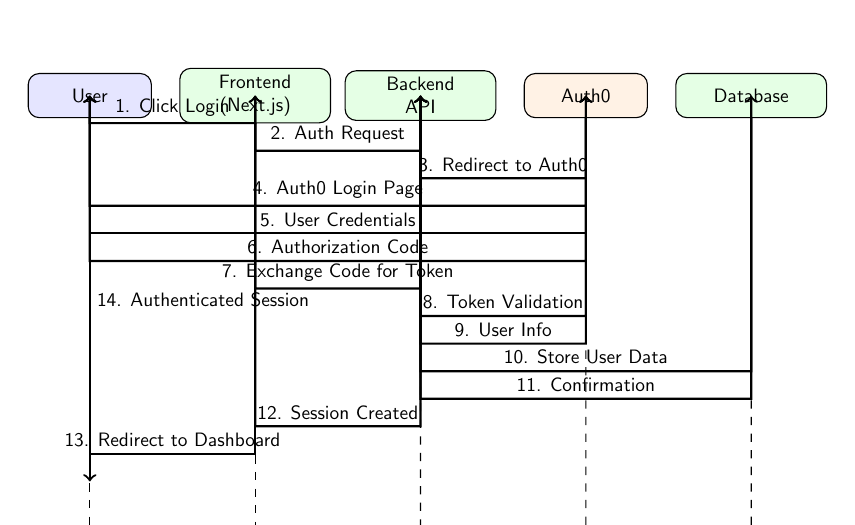
\begin{tikzpicture}[scale=0.7, transform shape]
    % Define styles
    \tikzstyle{actor} = [rectangle, draw=black, fill=blue!10, text width=2cm, text centered, rounded corners, minimum height=0.8cm]
    \tikzstyle{system} = [rectangle, draw=black, fill=green!10, text width=2.5cm, text centered, rounded corners, minimum height=0.8cm]
    \tikzstyle{external} = [rectangle, draw=black, fill=orange!10, text width=2cm, text centered, rounded corners, minimum height=0.8cm]
    
    % Actors and systems
    \node[actor] (user) at (0,0) {User};
    \node[system] (frontend) at (3,0) {Frontend\\(Next.js)};
    \node[system] (backend) at (6,0) {Backend\\API};
    \node[external] (auth0) at (9,0) {Auth0};
    \node[system] (database) at (12,0) {Database};
    
    % Lifelines
    \draw[dashed] (user) -- ++(0,-8);
    \draw[dashed] (frontend) -- ++(0,-8);
    \draw[dashed] (backend) -- ++(0,-8);
    \draw[dashed] (auth0) -- ++(0,-8);
    \draw[dashed] (database) -- ++(0,-8);
    
    % Sequence messages
    \draw[->, thick] (user) -- ++(0,-0.5) -- ++(3,0) node[midway, above] {1. Click Login} -- ++(0,0.5);
    \draw[->, thick] (frontend) -- ++(0,-1) -- ++(3,0) node[midway, above] {2. Auth Request} -- ++(0,1);
    \draw[->, thick] (backend) -- ++(0,-1.5) -- ++(3,0) node[midway, above] {3. Redirect to Auth0} -- ++(0,1.5);
    \draw[->, thick] (auth0) -- ++(0,-2) -- ++(-9,0) node[midway, above] {4. Auth0 Login Page} -- ++(0,2);
    \draw[->, thick] (user) -- ++(0,-2.5) -- ++(9,0) node[midway, above] {5. User Credentials} -- ++(0,2.5);
    \draw[->, thick] (auth0) -- ++(0,-3) -- ++(-9,0) node[midway, above] {6. Authorization Code} -- ++(0,3);
    \draw[->, thick] (frontend) -- ++(0,-3.5) -- ++(3,0) node[midway, above] {7. Exchange Code for Token} -- ++(0,3.5);
    \draw[->, thick] (backend) -- ++(0,-4) -- ++(3,0) node[midway, above] {8. Token Validation} -- ++(0,4);
    \draw[->, thick] (auth0) -- ++(0,-4.5) -- ++(-3,0) node[midway, above] {9. User Info} -- ++(0,4.5);
    \draw[->, thick] (backend) -- ++(0,-5) -- ++(6,0) node[midway, above] {10. Store User Data} -- ++(0,5);
    \draw[->, thick] (database) -- ++(0,-5.5) -- ++(-6,0) node[midway, above] {11. Confirmation} -- ++(0,5.5);
    \draw[->, thick] (backend) -- ++(0,-6) -- ++(-3,0) node[midway, above] {12. Session Created} -- ++(0,6);
    \draw[->, thick] (frontend) -- ++(0,-6.5) -- ++(-3,0) node[midway, above] {13. Redirect to Dashboard} -- ++(0,6.5);
    \draw[->, thick] (user) -- ++(0,-7) node[midway, right] {14. Authenticated Session};
    
\end{tikzpicture}
}
\caption{Complete Authentication Sequence Diagram}
\label{fig:auth-sequence}
\end{figure}

\subsubsection{API Request Flow Sequence}

\begin{figure}[H]
\centering
\resizebox{0.9\textwidth}{!}{%
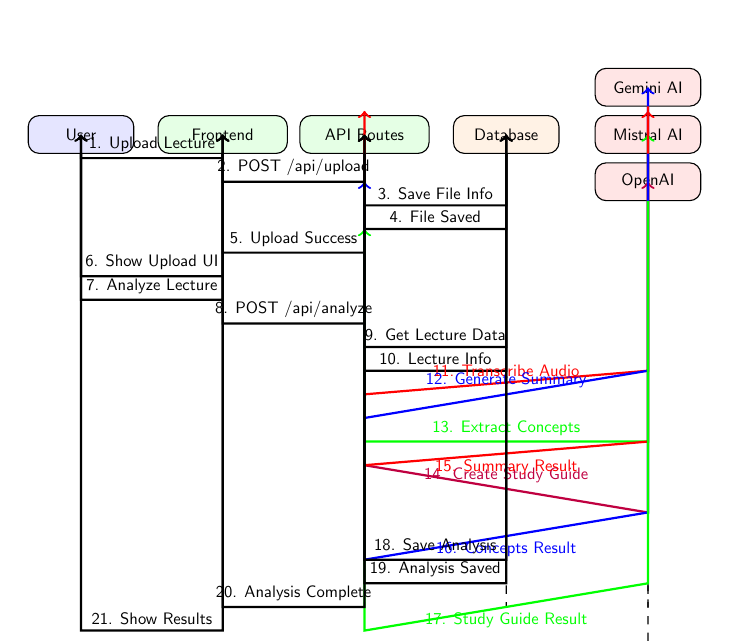
\begin{tikzpicture}[scale=0.6, transform shape]
    % Define styles
    \tikzstyle{actor} = [rectangle, draw=black, fill=blue!10, text width=2cm, text centered, rounded corners, minimum height=0.8cm]
    \tikzstyle{system} = [rectangle, draw=black, fill=green!10, text width=2.5cm, text centered, rounded corners, minimum height=0.8cm]
    \tikzstyle{data} = [rectangle, draw=black, fill=orange!10, text width=2cm, text centered, rounded corners, minimum height=0.8cm]
    \tikzstyle{ai} = [rectangle, draw=black, fill=red!10, text width=2cm, text centered, rounded corners, minimum height=0.8cm]
    
    % Actors and systems
    \node[actor] (user) at (0,0) {User};
    \node[system] (frontend) at (3,0) {Frontend};
    \node[system] (api) at (6,0) {API Routes};
    \node[data] (db) at (9,0) {Database};
    \node[ai] (aigemini) at (12,1) {Gemini AI};
    \node[ai] (aimistral) at (12,0) {Mistral AI};
    \node[ai] (aiopenai) at (12,-1) {OpenAI};
    
    % Lifelines
    \draw[dashed] (user) -- ++(0,-10);
    \draw[dashed] (frontend) -- ++(0,-10);
    \draw[dashed] (api) -- ++(0,-10);
    \draw[dashed] (db) -- ++(0,-10);
    \draw[dashed] (aigemini) -- ++(0,-10);
    \draw[dashed] (aimistral) -- ++(0,-10);
    \draw[dashed] (aiopenai) -- ++(0,-10);
    
    % Sequence messages for Lecture Analysis
    \draw[->, thick] (user) -- ++(0,-0.5) -- ++(3,0) node[midway, above] {1. Upload Lecture} -- ++(0,0.5);
    \draw[->, thick] (frontend) -- ++(0,-1) -- ++(3,0) node[midway, above] {2. POST /api/upload} -- ++(0,1);
    \draw[->, thick] (api) -- ++(0,-1.5) -- ++(3,0) node[midway, above] {3. Save File Info} -- ++(0,1.5);
    \draw[->, thick] (db) -- ++(0,-2) -- ++(-3,0) node[midway, above] {4. File Saved} -- ++(0,2);
    \draw[->, thick] (api) -- ++(0,-2.5) -- ++(-3,0) node[midway, above] {5. Upload Success} -- ++(0,2.5);
    \draw[->, thick] (frontend) -- ++(0,-3) -- ++(-3,0) node[midway, above] {6. Show Upload UI} -- ++(0,3);
    
    \draw[->, thick] (user) -- ++(0,-3.5) -- ++(3,0) node[midway, above] {7. Analyze Lecture} -- ++(0,3.5);
    \draw[->, thick] (frontend) -- ++(0,-4) -- ++(3,0) node[midway, above] {8. POST /api/analyze} -- ++(0,4);
    \draw[->, thick] (api) -- ++(0,-4.5) -- ++(3,0) node[midway, above] {9. Get Lecture Data} -- ++(0,4.5);
    \draw[->, thick] (db) -- ++(0,-5) -- ++(-3,0) node[midway, above] {10. Lecture Info} -- ++(0,5);
    
    % AI Processing calls
    \draw[->, thick, red] (api) -- ++(0,-5.5) -- ++(6,0.5) node[midway, above] {11. Transcribe Audio} -- ++(0,5.5);
    \draw[->, thick, blue] (api) -- ++(0,-6) -- ++(6,1) node[midway, above] {12. Generate Summary} -- ++(0,6);
    \draw[->, thick, green] (api) -- ++(0,-6.5) -- ++(6,0) node[midway, above] {13. Extract Concepts} -- ++(0,6.5);
    \draw[->, thick, purple] (api) -- ++(0,-7) -- ++(6,-1) node[midway, above] {14. Create Study Guide} -- ++(0,7);
    
    % AI Responses
    \draw[->, thick, red] (aigemini) -- ++(0,-7.5) -- ++(-6,-0.5) node[midway, below] {15. Summary Result} -- ++(0,7.5);
    \draw[->, thick, blue] (aimistral) -- ++(0,-8) -- ++(-6,-1) node[midway, below] {16. Concepts Result} -- ++(0,8);
    \draw[->, thick, green] (aiopenai) -- ++(0,-8.5) -- ++(-6,-1) node[midway, below] {17. Study Guide Result} -- ++(0,8.5);
    
    % Final steps
    \draw[->, thick] (api) -- ++(0,-9) -- ++(3,0) node[midway, above] {18. Save Analysis} -- ++(0,9);
    \draw[->, thick] (db) -- ++(0,-9.5) -- ++(-3,0) node[midway, above] {19. Analysis Saved} -- ++(0,9.5);
    \draw[->, thick] (api) -- ++(0,-10) -- ++(-3,0) node[midway, above] {20. Analysis Complete} -- ++(0,10);
    \draw[->, thick] (frontend) -- ++(0,-10.5) -- ++(-3,0) node[midway, above] {21. Show Results} -- ++(0,10.5);
    
\end{tikzpicture}
}
\caption{Lecture Analysis API Sequence Diagram}
\label{fig:api-sequence}
\end{figure}

\subsubsection{Session Management}

\begin{itemize}
    \item \textbf{Session Storage}: Sessions are stored using HTTP-only cookies
    \item \textbf{Token Validation}: Each API request validates the session token
    \item \textbf{Automatic Refresh}: Tokens are automatically refreshed when needed
    \item \textbf{Logout Process}: Sessions are properly invalidated on logout
\end{itemize}

\subsection{API Security}

\subsubsection{Security Measures}
\begin{itemize}
    \item \textbf{HTTPS Only}: All API endpoints require HTTPS in production
    \item \textbf{Input Validation}: All user inputs are validated and sanitized
    \item \textbf{Rate Limiting}: API endpoints implement rate limiting to prevent abuse
    \item \textbf{CORS Configuration}: Proper CORS headers for cross-origin requests
    \item \textbf{SQL Injection Prevention}: Parameterized queries for all database operations
\end{itemize}

\subsubsection{Error Handling}
\begin{itemize}
    \item \textbf{Standardized Responses}: Consistent error response format
    \item \textbf{Logging}: Comprehensive error logging for debugging
    \item \textbf{User-Friendly Messages}: Clear error messages for end users
    \item \textbf{Status Codes}: Proper HTTP status codes for different error types
\end{itemize}

\section{User Interface Components}

\subsection{UI/UX Architecture}

\subsubsection{User Interface Layout Diagram}

\begin{figure}[H]
\centering
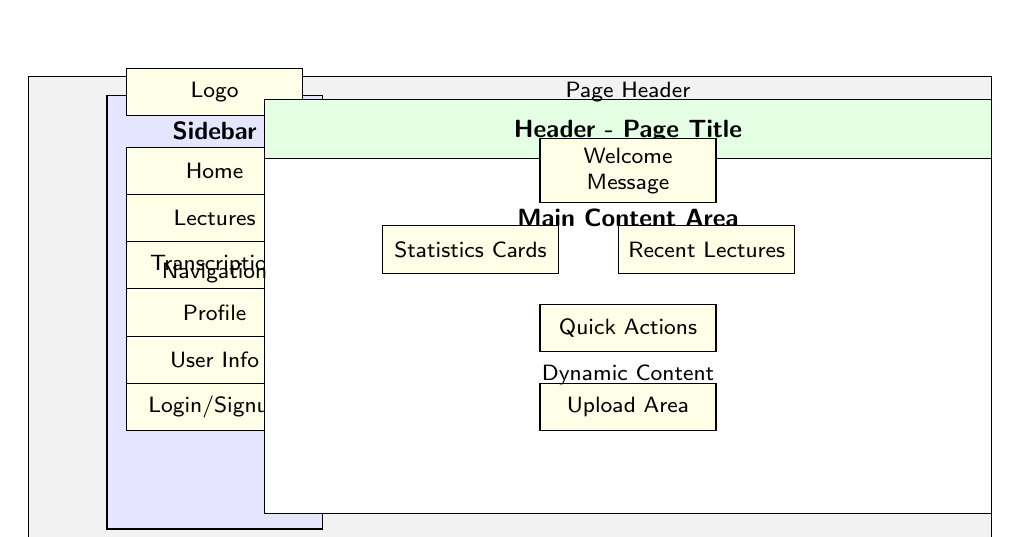
\begin{tikzpicture}[
    node distance=0.3cm,
    layout/.style={rectangle, draw=black, fill=gray!10, text width=12cm, text centered, minimum height=6cm},
    sidebar/.style={rectangle, draw=black, fill=blue!10, text width=2.5cm, text centered, minimum height=5.5cm},
    header/.style={rectangle, draw=black, fill=green!10, text width=9cm, text centered, minimum height=0.8cm},
    content/.style={rectangle, draw=black, fill=white, text width=9cm, text centered, minimum height=4.5cm},
    component/.style={rectangle, draw=black, fill=yellow!10, text width=2cm, text centered, minimum height=0.6cm, font=\footnotesize}
]

% Main Layout
\node[layout] (main) {};

% Sidebar
\node[sidebar] (sidebar) at (-3.75,0) {};
\node[font=\small\bfseries] at (-3.75,2.3) {Sidebar};
\node[component] (logo) at (-3.75,2.8) {Logo};
\node[component] (navhome) at (-3.75,1.8) {Home};
\node[component] (navlectures) at (-3.75,1.2) {Lectures};
\node[component] (navtranscription) at (-3.75,0.6) {Transcription};
\node[component] (navprofile) at (-3.75,0) {Profile};
\node[component] (userinfo) at (-3.75,-0.6) {User Info};
\node[component] (loginbtn) at (-3.75,-1.2) {Login/Signup};

% Main Content Area
\node[header] (header) at (1.5,2.3) {};
\node[font=\small\bfseries] at (1.5,2.3) {Header - Page Title};

\node[content] (content) at (1.5,-0.3) {};
\node[font=\small\bfseries] at (1.5,1.2) {Main Content Area};

% Content Components
\node[component] (welcome) at (1.5,1.8) {Welcome Message};
\node[component] (stats) at (-0.5,0.8) {Statistics Cards};
\node[component] (recent) at (2.5,0.8) {Recent Lectures};
\node[component] (actions) at (1.5,-0.2) {Quick Actions};
\node[component] (upload) at (1.5,-1.2) {Upload Area};

% Layout Labels
\node[font=\footnotesize, above of=sidebar, yshift=0.2cm] {Navigation};
\node[font=\footnotesize, above of=header, yshift=0.2cm] {Page Header};
\node[font=\footnotesize, below of=content, yshift=-0.2cm] {Dynamic Content};

\end{tikzpicture}
\caption{Complete UI Layout Architecture}
\label{fig:ui-layout}
\end{figure}

\subsubsection{User Flow Diagram}

\begin{figure}[H]
\centering
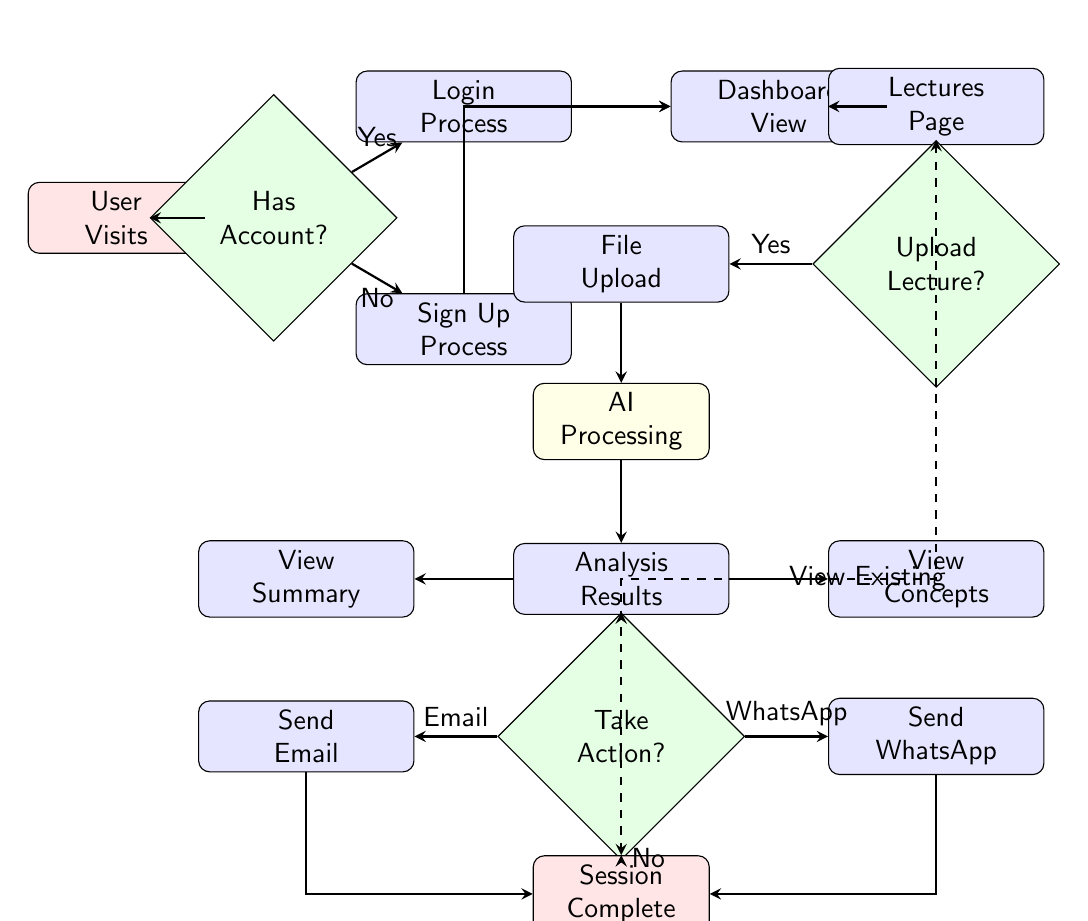
\begin{tikzpicture}[
    node distance=2cm,
    startstop/.style={rectangle, draw=black, fill=red!10, text width=2cm, text centered, rounded corners, minimum height=0.8cm},
    process/.style={rectangle, draw=black, fill=blue!10, text width=2.5cm, text centered, rounded corners, minimum height=0.8cm},
    decision/.style={diamond, draw=black, fill=green!10, text width=2cm, text centered, minimum height=0.8cm},
    data/.style={rectangle, draw=black, fill=yellow!10, text width=2cm, text centered, rounded corners, minimum height=0.8cm},
    arrow/.style={->,>=stealth,thick}
]

% Start
\node[startstop] (start) {User\\Visits};

% Authentication Flow
\node[decision, right of=start] (authcheck) {Has\\Account?};
\node[process, above right of=authcheck, xshift=1cm] (login) {Login\\Process};
\node[process, below right of=authcheck, xshift=1cm] (signup) {Sign Up\\Process};

% Main Application
\node[process, right of=login, xshift=2cm] (dashboard) {Dashboard\\View};
\node[process, right of=dashboard] (lectures) {Lectures\\Page};

% Upload Flow
\node[decision, below of=lectures] (uploaddecision) {Upload\\Lecture?};
\node[process, left of=uploaddecision, xshift=-2cm] (upload) {File\\Upload};
\node[data, below of=upload] (processing) {AI\\Processing};

% Analysis Flow
\node[process, below of=processing] (analysis) {Analysis\\Results};
\node[process, left of=analysis, xshift=-2cm] (summary) {View\\Summary};
\node[process, right of=analysis, xshift=2cm] (concepts) {View\\Concepts};

% Actions Flow
\node[decision, below of=analysis] (actiondecision) {Take\\Action?};
\node[process, left of=actiondecision, xshift=-2cm] (email) {Send\\Email};
\node[process, right of=actiondecision, xshift=2cm] (whatsapp) {Send\\WhatsApp};

% End
\node[startstop, below of=actiondecision] (end) {Session\\Complete};

% Connections
\draw[arrow] (start) -- (authcheck);
\draw[arrow] (authcheck) -- node[above] {Yes} (login);
\draw[arrow] (authcheck) -- node[below] {No} (signup);
\draw[arrow] (login) -- (dashboard);
\draw[arrow] (signup) |- (dashboard);
\draw[arrow] (dashboard) -- (lectures);
\draw[arrow] (lectures) -- (uploaddecision);
\draw[arrow] (uploaddecision) -- node[above] {Yes} (upload);
\draw[arrow] (upload) -- (processing);
\draw[arrow] (processing) -- (analysis);
\draw[arrow] (analysis) -- (summary);
\draw[arrow] (analysis) -- (concepts);
\draw[arrow] (analysis) -- (actiondecision);
\draw[arrow] (actiondecision) -- node[above] {Email} (email);
\draw[arrow] (actiondecision) -- node[above] {WhatsApp} (whatsapp);
\draw[arrow] (actiondecision) -- node[right] {No} (end);
\draw[arrow] (email) |- (end);
\draw[arrow] (whatsapp) |- (end);

% Alternative paths
\draw[arrow, dashed] (lectures) -- ++(0,-6) -| node[near start, right] {View Existing} (end);

\end{tikzpicture}
\caption{Complete User Flow Diagram}
\label{fig:user-flow}
\end{figure}

\subsubsection{Component Interaction Diagram}

\begin{figure}[H]
\centering
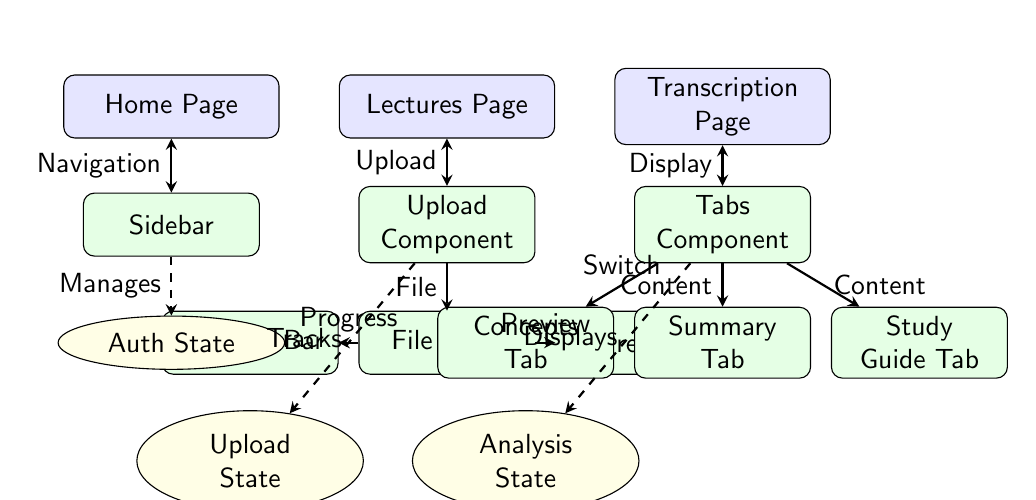
\begin{tikzpicture}[
    node distance=1.5cm,
    page/.style={rectangle, draw=black, fill=blue!10, text width=2.5cm, text centered, rounded corners, minimum height=0.8cm},
    component/.style={rectangle, draw=black, fill=green!10, text width=2cm, text centered, rounded corners, minimum height=0.8cm},
    state/.style={ellipse, draw=black, fill=yellow!10, text width=1.8cm, text centered, minimum height=0.6cm},
    arrow/.style={->,>=stealth,thick},
    bidirectional/.style={<->,>=stealth,thick}
]

% Pages
\node[page] (homepage) {Home Page};
\node[page, right of=homepage, xshift=2cm] (lecturespage) {Lectures Page};
\node[page, right of=lecturespage, xshift=2cm] (transcriptionpage) {Transcription Page};

% Components
\node[component, below of=homepage] (sidebar) {Sidebar};
\node[component, below of=lecturespage] (upload) {Upload Component};
\node[component, below of=transcriptionpage] (tabs) {Tabs Component};

% Sub-components
\node[component, below of=upload] (fileinput) {File Input};
\node[component, left of=fileinput, xshift=-1cm] (progress) {Progress Bar};
\node[component, right of=fileinput, xshift=1cm] (preview) {Preview};

\node[component, below of=tabs] (summary) {Summary Tab};
\node[component, left of=summary, xshift=-1cm] (concepts) {Concepts Tab};
\node[component, right of=summary, xshift=1cm] (studyguide) {Study Guide Tab};

% States
\node[state, below of=sidebar] (authstate) {Auth State};
\node[state, below of=progress] (uploadstate) {Upload State};
\node[state, below of=concepts] (analysisstate) {Analysis State};

% Connections
\draw[bidirectional] (homepage) -- (sidebar) node[midway, left] {Navigation};
\draw[bidirectional] (lecturespage) -- (upload) node[midway, left] {Upload};
\draw[bidirectional] (transcriptionpage) -- (tabs) node[midway, left] {Display};

\draw[arrow] (upload) -- (fileinput) node[midway, left] {File};
\draw[arrow] (fileinput) -- (progress) node[midway, above] {Progress};
\draw[arrow] (fileinput) -- (preview) node[midway, above] {Preview};

\draw[arrow] (tabs) -- (summary) node[midway, left] {Content};
\draw[arrow] (tabs) -- (concepts) node[midway, above] {Switch};
\draw[arrow] (tabs) -- (studyguide) node[midway, right] {Content};

\draw[arrow, dashed] (sidebar) -- (authstate) node[midway, left] {Manages};
\draw[arrow, dashed] (upload) -- (uploadstate) node[midway, left] {Tracks};
\draw[arrow, dashed] (tabs) -- (analysisstate) node[midway, left] {Displays};

\end{tikzpicture}
\caption{Component Interaction and State Management}
\label{fig:component-interaction}
\end{figure}

\begin{lstlisting}[caption=Root Layout Component]
import type { Metadata } from "next";
import { Inter } from "next/font/google";
import "./globals.css";
import Sidebar from "../components/Sidebar";

const inter = Inter({ subsets: ["latin"] });

export const metadata: Metadata = {
  title: "NurseNotes Clone",
  description: "AI-Powered Lecture Intelligence for Nursing Students",
};

export default function RootLayout({
  children,
}: Readonly<{
  children: React.ReactNode;
}>) {
  return (
    <html lang="en">
      <body className={`${inter.className} flex min-h-screen bg-slate-50`}>
        <Sidebar />
        <main className="flex-1 overflow-y-auto p-8">{children}</main>
      </body>
    </html>
  );
}
\end{lstlisting}

\subsection{Sidebar Component}

The sidebar provides navigation and user authentication status:

\begin{lstlisting}[caption=Sidebar Component Structure]
'use client';
import Link from 'next/link';
import { useEffect, useState } from 'react';

export default function Sidebar() {
  const [user, setUser] = useState<{ name: string; email: string; role: string } | null>(null);

  useEffect(() => {
    let mounted = true;
    fetch('/api/auth/me')
      .then((r) => (r.ok ? r.json() : null))
      .then((u) => {
        if (mounted) setUser(u || null);
      })
      .catch(() => {});
    return () => {
      mounted = false;
    };
  }, []);

  return (
    <div className="w-72 bg-white border-r border-slate-200 text-slate-700 p-6 flex flex-col h-screen sticky top-0">
      {/* Sidebar content */}
    </div>
  );
}
\end{lstlisting}

\subsection{Tabs Component}

A reusable tab interface for displaying different content sections:

\begin{lstlisting}[caption=Tabs Component]
'use client';
import { useState } from 'react';

interface Tab {
  name: string;
  content: React.ReactNode;
}

interface TabsProps {
  tabs: Tab[];
}

export default function Tabs({ tabs }: TabsProps) {
  const [activeTab, setActiveTab] = useState(0);

  return (
    <div>
      <div className="flex border-b border-slate-200 mb-6">
        {tabs.map((tab, index) => (
          <button
            key={index}
            onClick={() => setActiveTab(index)}
            className={`px-6 py-3 font-medium text-sm border-b-2 transition-colors ${
              activeTab === index
                ? 'border-indigo-500 text-indigo-600'
                : 'border-transparent text-slate-500 hover:text-slate-700'
            }`}
          >
            {tab.name}
          </button>
        ))}
      </div>
      <div>{tabs[activeTab].content}</div>
    </div>
  );
}
\end{lstlisting}

\subsection{File Upload Component}

Drag-and-drop file upload with progress indication:

\begin{lstlisting}[caption=File Upload Component]
'use client';
import { useState, useCallback } from 'react';

export default function FileUpload() {
  const [isUploading, setIsUploading] = useState(false);
  const [uploadProgress, setUploadProgress] = useState(0);

  const handleFileUpload = useCallback(async (file: File) => {
    setIsUploading(true);
    setUploadProgress(0);

    const formData = new FormData();
    formData.append('file', file);

    try {
      const response = await fetch('/api/upload', {
        method: 'POST',
        body: formData,
      });

      if (response.ok) {
        const result = await response.json();
        console.log('Upload successful:', result);
      }
    } catch (error) {
      console.error('Upload failed:', error);
    } finally {
      setIsUploading(false);
      setUploadProgress(0);
    }
  }, []);

  return (
    <div className="border-2 border-dashed border-slate-300 rounded-lg p-8 text-center">
      {/* Upload UI */}
    </div>
  );
}
\end{lstlisting}

\section{AI Integration}

\subsection{AI Service Architecture}

The application integrates multiple AI services for comprehensive content analysis:

\subsubsection{AI Processing Pipeline Diagram}

\begin{figure}[H]
\centering
\resizebox{0.85\textwidth}{!}{%
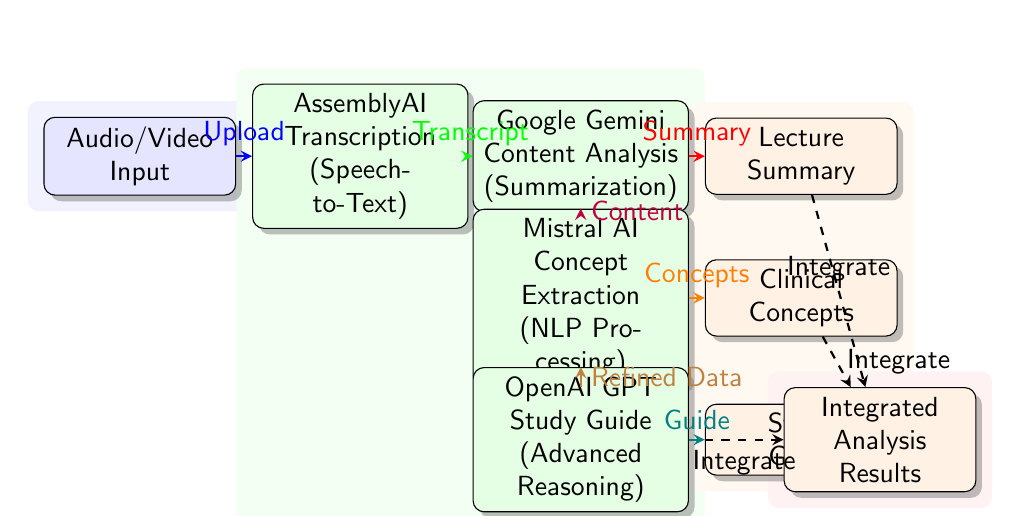
\begin{tikzpicture}[
    node distance=1.8cm,
    input/.style={rectangle, draw=black, fill=blue!10, text width=2.2cm, text centered, rounded corners, minimum height=0.8cm, drop shadow},
    process/.style={rectangle, draw=black, fill=green!10, text width=2.5cm, text centered, rounded corners, minimum height=0.8cm, drop shadow},
    output/.style={rectangle, draw=black, fill=orange!10, text width=2.2cm, text centered, rounded corners, minimum height=0.8cm, drop shadow},
    arrow/.style={->,>=stealth,thick}
]

% Input
\node[input] (audio) {Audio/Video\\Input};

% Processing Steps
\node[process, right of=audio, xshift=1cm] (assembly) {AssemblyAI\\Transcription\\(Speech-to-Text)};
\node[process, right of=assembly, xshift=1cm] (gemini) {Google Gemini\\Content Analysis\\(Summarization)};
\node[process, below of=gemini] (mistral) {Mistral AI\\Concept Extraction\\(NLP Processing)};
\node[process, below of=mistral] (openai) {OpenAI GPT\\Study Guide\\(Advanced Reasoning)};

% Outputs
\node[output, right of=gemini, xshift=1cm] (summary) {Lecture\\Summary};
\node[output, right of=mistral, xshift=1cm] (concepts) {Clinical\\Concepts};
\node[output, right of=openai, xshift=1cm] (studyguide) {Study\\Guide};

% Final Integration
\node[output, below of=concepts, xshift=1cm] (integrated) {Integrated\\Analysis\\Results};

% Connections
\draw[arrow, blue] (audio) -- (assembly) node[midway, above] {Upload};
\draw[arrow, green] (assembly) -- (gemini) node[midway, above] {Transcript};
\draw[arrow, red] (gemini) -- (summary) node[midway, above] {Summary};
\draw[arrow, purple] (gemini) -- (mistral) node[midway, right] {Content};
\draw[arrow, orange] (mistral) -- (concepts) node[midway, above] {Concepts};
\draw[arrow, brown] (mistral) -- (openai) node[midway, right] {Refined Data};
\draw[arrow, teal] (openai) -- (studyguide) node[midway, above] {Guide};

% Integration arrows
\draw[arrow, dashed] (summary) -- (integrated) node[midway, above] {Integrate};
\draw[arrow, dashed] (concepts) -- (integrated) node[midway, right] {Integrate};
\draw[arrow, dashed] (studyguide) -- (integrated) node[midway, below] {Integrate};

% Background regions
\begin{scope}[on background layer]
    \node[fit=(audio), fill=blue!5, rounded corners, inner sep=0.2cm] {};
    \node[fit=(assembly)(gemini)(mistral)(openai), fill=green!5, rounded corners, inner sep=0.2cm] {};
    \node[fit=(summary)(concepts)(studyguide), fill=orange!5, rounded corners, inner sep=0.2cm] {};
    \node[fit=(integrated), fill=red!5, rounded corners, inner sep=0.2cm] {};
\end{scope}

\end{tikzpicture}
}
\caption{Complete AI Processing Pipeline}
\label{fig:ai-pipeline}
\end{figure}

\subsubsection{AI Service Integration Architecture}

\begin{figure}[H]
\centering
\resizebox{0.85\textwidth}{!}{%
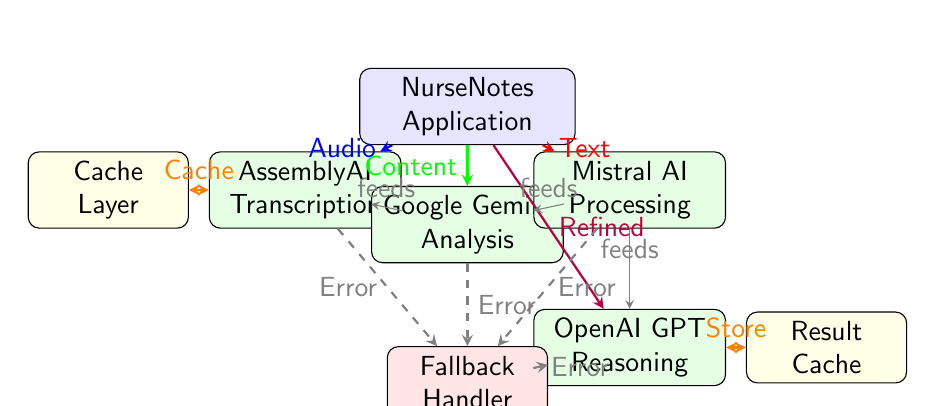
\begin{tikzpicture}[
    node distance=1.5cm,
    app/.style={rectangle, draw=black, fill=blue!10, text width=2.5cm, text centered, rounded corners, minimum height=0.8cm},
    service/.style={rectangle, draw=black, fill=green!10, text width=2.2cm, text centered, rounded corners, minimum height=0.8cm},
    cache/.style={rectangle, draw=black, fill=yellow!10, text width=1.8cm, text centered, rounded corners, minimum height=0.8cm},
    error/.style={rectangle, draw=black, fill=red!10, text width=1.8cm, text centered, rounded corners, minimum height=0.8cm},
    arrow/.style={->,>=stealth,thick},
    bidirectional/.style={<->,>=stealth,thick}
]

% Application Layer
\node[app] (nurseapp) {NurseNotes\\Application};

% AI Services
\node[service, below left of=nurseapp, xshift=-1cm] (assembly) {AssemblyAI\\Transcription};
\node[service, below of=nurseapp] (gemini) {Google Gemini\\Analysis};
\node[service, below right of=nurseapp, xshift=1cm] (mistral) {Mistral AI\\Processing};
\node[service, below of=mistral, yshift=-0.5cm] (openai) {OpenAI GPT\\Reasoning};

% Supporting Services
\node[cache, left of=assembly, xshift=-1cm] (cache1) {Cache\\Layer};
\node[cache, right of=openai, xshift=1cm] (cache2) {Result\\Cache};
\node[error, below of=gemini, yshift=-0.5cm] (fallback) {Fallback\\Handler};

% Connections
\draw[arrow, blue] (nurseapp) -- (assembly) node[midway, left] {Audio};
\draw[arrow, green] (nurseapp) -- (gemini) node[midway, left] {Content};
\draw[arrow, red] (nurseapp) -- (mistral) node[midway, right] {Text};
\draw[arrow, purple] (nurseapp) -- (openai) node[midway, right] {Refined};

\draw[bidirectional, orange] (assembly) -- (cache1) node[midway, above] {Cache};
\draw[bidirectional, orange] (openai) -- (cache2) node[midway, above] {Store};

\draw[arrow, dashed, gray] (assembly) -- (fallback) node[midway, left] {Error};
\draw[arrow, dashed, gray] (gemini) -- (fallback) node[midway, right] {Error};
\draw[arrow, dashed, gray] (mistral) -- (fallback) node[midway, right] {Error};
\draw[arrow, dashed, gray] (openai) -- (fallback) node[midway, right] {Error};

% Service Dependencies
\draw[arrow, thin, gray] (assembly) -- (gemini) node[midway, above] {feeds};
\draw[arrow, thin, gray] (gemini) -- (mistral) node[midway, above] {feeds};
\draw[arrow, thin, gray] (mistral) -- (openai) node[midway, above] {feeds};

\end{tikzpicture}
}
\caption{AI Service Integration with Caching and Fallback}
\label{fig:ai-integration}
\end{figure}

\subsubsection{AI Performance Metrics}

\begin{figure}[H]
\centering
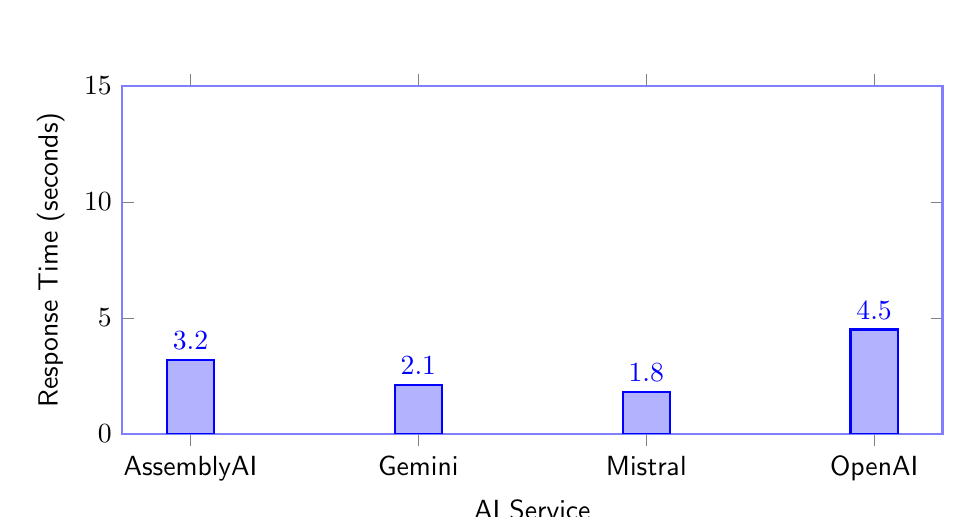
\begin{tikzpicture}
\begin{axis}[
    ybar,
    width=12cm,
    height=6cm,
    ylabel={Response Time (seconds)},
    xlabel={AI Service},
    symbolic x coords={AssemblyAI,Gemini,Mistral,OpenAI},
    xtick=data,
    nodes near coords,
    nodes near coords align={vertical},
    ymin=0,
    ymax=15,
    bar width=0.6cm,
    fill=blue!30,
    draw=blue!50,
    thick
]
\addplot coordinates {(AssemblyAI,3.2) (Gemini,2.1) (Mistral,1.8) (OpenAI,4.5)};
\end{axis}
\end{tikzpicture}
\caption{AI Service Performance Comparison}
\label{fig:ai-performance}
\end{figure}

\subsection{Analysis API Implementation}

\begin{lstlisting}[caption=AI Analysis Implementation]
import { GoogleGenerativeAI } from '@google/generative-ai';
import MistralClient from '@mistralai/mistralai';
import OpenAI from 'openai';
import { AssemblyAI } from 'assemblyai';

const genAI = new GoogleGenerativeAI(process.env.GOOGLE_GENERATIVE_AI_API_KEY);
const mistral = new MistralClient(process.env.MISTRAL_API_KEY);
const openai = new OpenAI({ apiKey: process.env.OPENAI_API_KEY });
const assemblyai = new AssemblyAI({ apiKey: process.env.ASSEMBLYAI_API_KEY });

export async function analyzeLecture(audioUrl: string) {
  // Step 1: Transcribe audio
  const transcript = await assemblyai.transcripts.transcribe({
    audio: audioUrl,
    language_code: 'en_us'
  });

  // Step 2: Generate summary with Gemini
  const model = genAI.getGenerativeModel({ model: 'gemini-pro' });
  const summaryPrompt = `Summarize this lecture transcript for nursing students: ${transcript.text}`;
  const summary = await model.generateContent(summaryPrompt);

  // Step 3: Extract clinical concepts with Mistral
  const conceptsPrompt = `Extract key clinical concepts from: ${transcript.text}`;
  const concepts = await mistral.chat({
    model: 'mistral-medium',
    messages: [{ role: 'user', content: conceptsPrompt }]
  });

  // Step 4: Generate study guide with OpenAI
  const studyGuidePrompt = `Create a study guide for nursing students based on: ${transcript.text}`;
  const studyGuide = await openai.chat.completions.create({
    model: 'gpt-4',
    messages: [{ role: 'user', content: studyGuidePrompt }]
  });

  return {
    summary: summary.response.text(),
    clinicalConcepts: JSON.parse(concepts.choices[0].message.content),
    studyGuide: studyGuide.choices[0].message.content
  };
}
\end{lstlisting}

\subsection{Error Handling and Fallbacks}

\subsubsection{AI Service Reliability}
\begin{itemize}
    \item \textbf{Retry Logic}: Automatic retries with exponential backoff
    \item \textbf{Fallback Services}: Alternative AI providers when primary fails
    \item \textbf{Graceful Degradation}: Partial results when some services fail
    \item \textbf{User Feedback}: Clear error messages and retry options
\end{itemize}

\subsubsection{Performance Optimization}
\begin{itemize}
    \item \textbf{Caching}: Cache analysis results to avoid reprocessing
    \item \textbf{Streaming}: Process large files in chunks
    \item \textbf{Async Processing}: Background processing for long-running tasks
    \item \textbf{Rate Limiting}: Respect AI service rate limits
\end{itemize}

\section{Deployment and CI/CD}

\subsection{Deployment Architecture}

\subsubsection{Cloud Deployment Architecture}

\begin{figure}[H]
\centering
\resizebox{0.85\textwidth}{!}{%
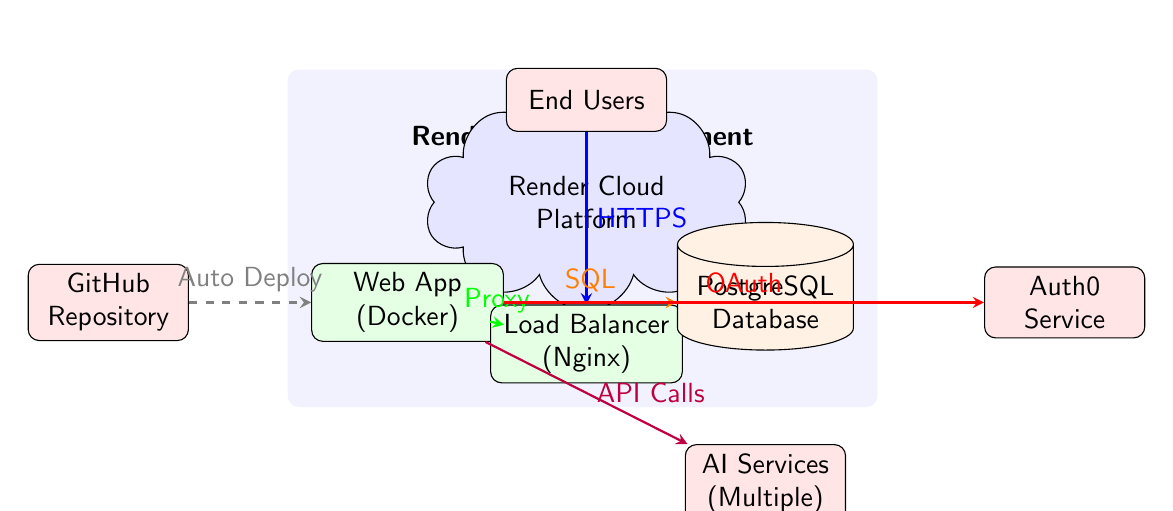
\begin{tikzpicture}[
    node distance=1.8cm,
    cloudnode/.style={cloud, draw=black, fill=blue!10, text width=2.5cm, text centered, minimum height=1.5cm, aspect=2},
    service/.style={rectangle, draw=black, fill=green!10, text width=2.2cm, text centered, rounded corners, minimum height=0.8cm},
    database/.style={cylinder, draw=black, fill=orange!10, text width=2cm, text centered, minimum height=0.8cm, shape border rotate=90, aspect=0.25},
    external/.style={rectangle, draw=black, fill=red!10, text width=1.8cm, text centered, rounded corners, minimum height=0.8cm},
    arrow/.style={->,>=stealth,thick}
]

% Cloud Provider
\node[cloudnode] (render) {Render Cloud\\Platform};

% Services within Render
\node[service, below left of=render, xshift=-1cm] (webapp) {Web App\\(Docker)};
\node[service, below of=render] (nginx) {Load Balancer\\(Nginx)};
\node[database, below right of=render, xshift=1cm] (postgres) {PostgreSQL\\Database};

% External Services
\node[external, left of=webapp, xshift=-2cm] (github) {GitHub\\Repository};
\node[external, right of=postgres, xshift=2cm] (auth0ext) {Auth0\\Service};
\node[external, below of=postgres, yshift=-0.5cm] (aiservices) {AI Services\\(Multiple)};

% User Access
\node[external, above of=render, yshift=-0.5cm] (users) {End Users};

% Connections
\draw[arrow, blue] (users) -- (nginx) node[midway, right] {HTTPS};
\draw[arrow, green] (nginx) -- (webapp) node[midway, above] {Proxy};
\draw[arrow, orange] (webapp) -- (postgres) node[midway, above] {SQL};
\draw[arrow, red] (webapp) -- (auth0ext) node[midway, above] {OAuth};
\draw[arrow, purple] (webapp) -- (aiservices) node[midway, right] {API Calls};

% CI/CD Connection
\draw[arrow, dashed, gray] (github) -- (webapp) node[midway, above] {Auto Deploy};

% Background regions
\begin{scope}[on background layer]
    \node[fit=(render)(webapp)(nginx)(postgres), fill=blue!5, rounded corners, inner sep=0.3cm] (cloudregion) {};
    \node[above of=cloudregion, yshift=-0.5cm] {\textbf{Render Cloud Environment}};
\end{scope}

\end{tikzpicture}
\caption{Complete Cloud Deployment Architecture}
\label{fig:deployment-architecture}
\end{figure}

\subsubsection{CI/CD Pipeline Architecture}

\begin{figure}[H]
\centering
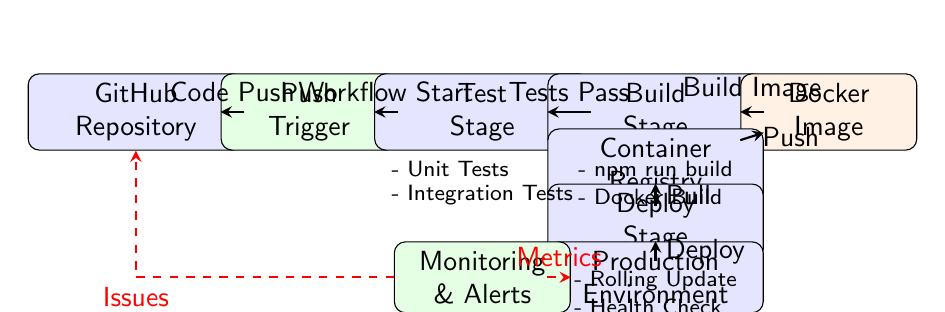
\begin{tikzpicture}[
    node distance=1.2cm,
    stage/.style={rectangle, draw=black, fill=blue!10, text width=2.5cm, text centered, rounded corners, minimum height=0.8cm},
    action/.style={rectangle, draw=black, fill=green!10, text width=2cm, text centered, rounded corners, minimum height=0.8cm},
    artifact/.style={rectangle, draw=black, fill=orange!10, text width=2cm, text centered, rounded corners, minimum height=0.8cm},
    arrow/.style={->,>=stealth,thick}
]

% Git Repository
\node[stage] (git) {GitHub\\Repository};

% CI/CD Stages
\node[action, right of=git, xshift=1cm] (trigger) {Push\\Trigger};
\node[stage, right of=trigger, xshift=1cm] (test) {Test\\Stage};
\node[stage, right of=test, xshift=1cm] (build) {Build\\Stage};
\node[artifact, right of=build, xshift=1cm] (docker) {Docker\\Image};
\node[stage, below of=build, yshift=0.5cm] (registry) {Container\\Registry};
\node[stage, below of=registry, yshift=0.5cm] (deploy) {Deploy\\Stage};
\node[stage, below of=deploy, yshift=0.5cm] (production) {Production\\Environment};

% Monitoring
\node[action, left of=production, xshift=-1cm] (monitor) {Monitoring\\\& Alerts};

% Connections
\draw[arrow] (git) -- (trigger) node[midway, above] {Code Push};
\draw[arrow] (trigger) -- (test) node[midway, above] {Workflow Start};
\draw[arrow] (test) -- (build) node[midway, above] {Tests Pass};
\draw[arrow] (build) -- (docker) node[midway, above] {Build Image};
\draw[arrow] (docker) -- (registry) node[midway, right] {Push};
\draw[arrow] (registry) -- (deploy) node[midway, right] {Pull};
\draw[arrow] (deploy) -- (production) node[midway, right] {Deploy};

% Monitoring feedback
\draw[arrow, dashed, red] (production) -- (monitor) node[midway, above] {Metrics};
\draw[arrow, dashed, red] (monitor) -| (git) node[midway, below] {Issues};

% Stage details
\node[font=\footnotesize, below of=test, yshift=0.3cm] {\shortstack[l]{- Unit Tests\\- Integration Tests}};
\node[font=\footnotesize, below of=build, yshift=0.3cm] {\shortstack[l]{- npm run build\\- Docker Build}};
\node[font=\footnotesize, below of=deploy, yshift=0.3cm] {\shortstack[l]{- Rolling Update\\- Health Check}};

\end{tikzpicture}
\caption{Complete CI/CD Pipeline with Monitoring}
\label{fig:cicd-pipeline}
\end{figure}

\subsubsection{Docker Container Architecture}

\begin{figure}[H]
\centering
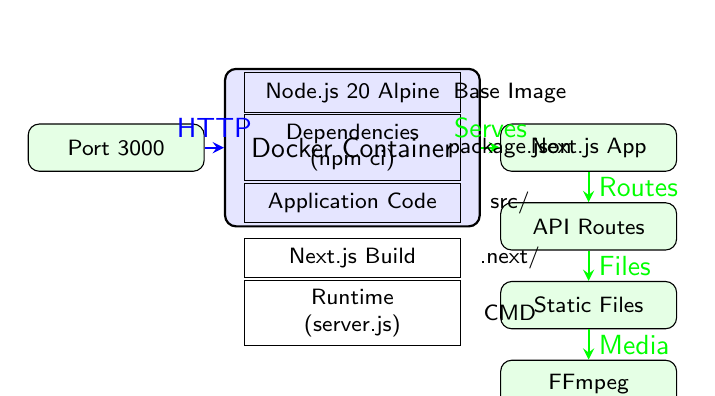
\begin{tikzpicture}[
    node distance=1cm,
    container/.style={rectangle, draw=black, fill=blue!10, text width=3cm, text centered, rounded corners, minimum height=2cm, thick},
    layer/.style={rectangle, draw=black, text width=2.5cm, text centered, minimum height=0.5cm, font=\footnotesize},
    app/.style={rectangle, draw=black, fill=green!10, text width=2cm, text centered, rounded corners, minimum height=0.6cm, font=\footnotesize},
    arrow/.style={->,>=stealth,thick}
]

% Docker Container
\node[container] (docker) {Docker Container};

% Container Layers
\node[layer, above of=docker, yshift=-0.3cm] (nodejs) {Node.js 20 Alpine};
\node[layer, below of=nodejs, yshift=0.3cm] (dependencies) {Dependencies\\(npm ci)};
\node[layer, below of=dependencies, yshift=0.3cm] (appcode) {Application Code};
\node[layer, below of=appcode, yshift=0.3cm] (build) {Next.js Build};
\node[layer, below of=build, yshift=0.3cm] (runtime) {Runtime\\(server.js)};

% Application Components
\node[app, right of=docker, xshift=2cm] (nextapp) {Next.js App};
\node[app, below of=nextapp] (api) {API Routes};
\node[app, below of=api] (static) {Static Files};
\node[app, below of=static] (ffmpeg) {FFmpeg};

% External Connections
\node[app, left of=docker, xshift=-2cm] (port3000) {Port 3000};

% Connections
\draw[arrow, blue] (port3000) -- (docker) node[midway, above] {HTTP};
\draw[arrow, green] (docker) -- (nextapp) node[midway, above] {Serves};
\draw[arrow, green] (nextapp) -- (api) node[midway, right] {Routes};
\draw[arrow, green] (api) -- (static) node[midway, right] {Files};
\draw[arrow, green] (static) -- (ffmpeg) node[midway, right] {Media};

% Container annotations
\node[font=\footnotesize, right of=nodejs, xshift=1cm] {Base Image};
\node[font=\footnotesize, right of=dependencies, xshift=1cm] {package.json};
\node[font=\footnotesize, right of=appcode, xshift=1cm] {src/};
\node[font=\footnotesize, right of=build, xshift=1cm] {.next/};
\node[font=\footnotesize, right of=runtime, xshift=1cm] {CMD};

\end{tikzpicture}
\caption{Docker Container Internal Architecture}
\label{fig:docker-architecture}
\end{figure}

The application is containerized using Docker for consistent deployment:

\begin{lstlisting}[caption=Dockerfile Configuration]
FROM node:20-alpine AS base

# Install dependencies only when needed
FROM base AS deps
RUN apk add --no-cache libc6-compat
WORKDIR /app

# Install dependencies
COPY package.json package-lock.json* ./
RUN npm ci

# Rebuild the source code only when needed
FROM base AS builder
WORKDIR /app
COPY --from=deps /app/node_modules ./node_modules
COPY . .

# Install FFmpeg for build
RUN apk add --no-cache ffmpeg

# Next.js configuration
ENV NODE_ENV=production
RUN npm run build

# Production image
FROM base AS runner
WORKDIR /app

ENV NODE_ENV=production
RUN addgroup --system --gid 1001 nodejs
RUN adduser --system --uid 1001 nextjs

COPY --from=builder /app/public ./public
COPY --from=builder --chown=nextjs:nodejs /app/.next/standalone ./
COPY --from=builder --chown=nextjs:nodejs /app/.next/static ./.next/static

USER nextjs
EXPOSE 3000
ENV PORT=3000
ENV HOSTNAME="0.0.0.0"

CMD ["node", "server.js"]
\end{lstlisting}

\subsection{CI/CD Pipeline}

The application uses GitHub Actions for automated testing and deployment:

\begin{lstlisting}[caption=GitHub Actions Workflow]
name: Docker CI/CD

on:
  push:
    branches: [ main, develop ]
  pull_request:
    branches: [ main ]

env:
  REGISTRY: ghcr.io
  IMAGE_NAME: ${{ github.repository }}

jobs:
  test:
    runs-on: ubuntu-latest
    steps:
    - uses: actions/checkout@v4

    - name: Setup Node.js
      uses: actions/setup-node@v4
      with:
        node-version: '20'
        cache: 'npm'

    - name: Install dependencies
      run: npm ci

    - name: Run linting
      run: npm run lint

    - name: Run tests
      run: npm run test

  build-and-push:
    needs: test
    runs-on: ubuntu-latest
    permissions:
      contents: read
      packages: write

    steps:
    - name: Checkout repository
      uses: actions/checkout@v4

    - name: Log in to Container Registry
      uses: docker/login-action@v3
      with:
        registry: ${{ env.REGISTRY }}
        username: ${{ github.actor }}
        password: ${{ secrets.GITHUB_TOKEN }}

    - name: Build and push Docker image
      uses: docker/build-push-action@v5
      with:
        context: .
        push: true
        tags: ${{ steps.meta.outputs.tags }}
        labels: ${{ steps.meta.outputs.labels }}

  deploy:
    needs: build-and-push
    runs-on: ubuntu-latest
    if: github.ref == 'refs/heads/main'

    steps:
    - name: Deploy to production
      uses: appleboy/ssh-action@v1.0.3
      with:
        host: ${{ secrets.DEPLOY_HOST }}
        username: ${{ secrets.DEPLOY_USER }}
        key: ${{ secrets.DEPLOY_SSH_KEY }}
        script: |
          cd /opt/app
          docker-compose pull
          docker-compose up -d
          docker system prune -f
\end{lstlisting}

\subsection{Environment Configuration}

\begin{table}[H]
\centering
\caption{Environment Variables}
\label{tab:env-vars}
\scriptsize
\begin{tabular}{@{}>{\raggedright\arraybackslash}p{4.4cm}>{\raggedright\arraybackslash}p{8.0cm}>{\raggedright\arraybackslash}p{1.6cm}@{}}
\toprule
\textbf{Variable} & \textbf{Description} & \textbf{Required} \\
\midrule
NODE\_ENV & Environment mode & Yes \\
PORT & Server port & No (default: 3000) \\
HOSTNAME & Server hostname & No (default: 0.0.0.0) \\
DATABASE\_URL & PostgreSQL connection string & Yes \\
AUTH0\_SECRET & Auth0 client secret & Yes \\
AUTH0\_BASE\_URL & Application base URL & Yes \\
AUTH0\_ISSUER\_BASE\_URL & Auth0 domain URL & Yes \\
AUTH0\_CLIENT\_ID & Auth0 client ID & Yes \\
AUTH0\_CLIENT\_SECRET & Auth0 client secret & Yes \\
GOOGLE\_\allowbreak{}GENERATIVE\_\allowbreak{}AI\_\allowbreak{}API\_\allowbreak{}KEY & Google Gemini API key & Yes \\
MISTRAL\_API\_KEY & Mistral AI API key & Yes \\
OPENAI\_API\_KEY & OpenAI API key & Yes \\
ASSEMBLYAI\_API\_KEY & AssemblyAI API key & Yes \\
TWILIO\_ACCOUNT\_SID & Twilio account SID & Yes \\
TWILIO\_AUTH\_TOKEN & Twilio auth token & Yes \\
EMAIL\_HOST & SMTP host & Yes \\
EMAIL\_PORT & SMTP port & Yes \\
EMAIL\_USER & SMTP username & Yes \\
EMAIL\_PASS & SMTP password & Yes \\
\bottomrule
\end{tabular}
\normalsize
\end{table}

\subsection{Render Deployment}

\subsubsection{Deployment Steps}
\begin{enumerate}
    \item \textbf{Create Render Account}: Sign up at render.com
    \item \textbf{Connect Repository}: Link GitHub repository
    \item \textbf{Configure Service}: Set up Docker web service
    \item \textbf{Environment Variables}: Add all required environment variables
    \item \textbf{Deploy}: Automatic deployment on push to main branch
\end{enumerate}

\subsubsection{Render Configuration}
\begin{itemize}
    \item \textbf{Service Type}: Docker Web Service
    \item \textbf{Instance Type}: Free tier (or paid for production)
    \item \textbf{Auto-Deploy}: Enabled for main branch
    \item \textbf{Health Check}: /api/health endpoint
    \item \textbf{Custom Domain}: Configure domain name if needed
\end{itemize}

\section{Development Guide}

\subsection{Getting Started}

\begin{enumerate}
    \item \textbf{Clone the repository:}
    \begin{lstlisting}[language=bash]
    git clone https://github.com/yourusername/esrunNotes.git
    cd esrunNotes
    \end{lstlisting}

    \item \textbf{Install dependencies:}
    \begin{lstlisting}[language=bash]
    npm install
    \end{lstlisting}

    \item \textbf{Set up environment variables:}
    \begin{lstlisting}[language=bash]
    cp .env.example .env.local
    # Edit .env.local with your API keys
    \end{lstlisting}

    \item \textbf{Start development server:}
    \begin{lstlisting}[language=bash]
    npm run dev
    \end{lstlisting}
\end{enumerate}

\subsection{Key Development Concepts}

\subsubsection{1. Next.js App Router}
The application uses Next.js 14 App Router for file-based routing:
\begin{itemize}
    \item \code{app/page.tsx} - Home page
    \item \code{app/lectures/page.tsx} - Lectures listing
    \item \code{app/transcription/page.tsx} - Analysis results
    \item \code{app/api/*/route.ts} - API endpoints
\end{itemize}

\subsubsection{2. Authentication with Auth0}
Secure authentication using Next.js Auth0 integration:
\begin{lstlisting}[caption=Auth0 Configuration]
import { getSession } from '@auth0/nextjs-auth0';

export async function GET(request: NextRequest) {
  const res = new NextResponse();
  const session = await getSession(request, res);

  if (!session?.user?.email) {
    return NextResponse.json({ error: 'Not authenticated' }, { status: 401 });
  }

  // User is authenticated, proceed with logic
}
\end{lstlisting}

\subsubsection{3. Database Operations}
PostgreSQL integration with connection pooling:
\begin{lstlisting}[caption=Database Operations]
import { db, initDb } from '../../../lib/db';

export async function GET() {
  await initDb();
  const p = db();

  const result = await p.query('SELECT * FROM lectures WHERE user_id = $1', [userId]);
  return NextResponse.json(result.rows);
}
\end{lstlisting}

\subsubsection{4. File Upload Handling}
Multi-part file upload with Next.js API routes:
\begin{lstlisting}[caption=File Upload API]
import { writeFile } from 'fs/promises';
import { NextRequest, NextResponse } from 'next/server';

export async function POST(request: NextRequest) {
  const data = await request.formData();
  const file = data.get('file') as File;

  if (!file) {
    return NextResponse.json({ error: 'No file provided' }, { status: 400 });
  }

  const bytes = await file.arrayBuffer();
  const buffer = Buffer.from(bytes);

  // Save file to disk or cloud storage
  const filePath = `/uploads/${file.name}`;
  await writeFile(filePath, buffer);

  return NextResponse.json({ filePath });
}
\end{lstlisting}

\subsubsection{5. AI Integration Patterns}
Multi-service AI integration with error handling:
\begin{lstlisting}[caption=AI Service Integration]
async function analyzeContent(content: string) {
  try {
    // Primary AI service
    const primaryResult = await callPrimaryAI(content);

    // Fallback to secondary AI service
    if (!primaryResult) {
      return await callSecondaryAI(content);
    }

    return primaryResult;
  } catch (error) {
    console.error('AI analysis failed:', error);
    throw new Error('Analysis service unavailable');
  }
}
\end{lstlisting}

\subsection{Testing Strategy}

The application uses Vitest for unit testing:
\begin{lstlisting}[caption=Example Test]
import { describe, it, expect } from 'vitest';
import { analyzeLecture } from '../lib/ai';

describe('AI Analysis', () => {
  it('should analyze lecture content', async () => {
    const result = await analyzeLecture('sample-audio-url');
    expect(result).toHaveProperty('summary');
    expect(result).toHaveProperty('clinicalConcepts');
    expect(result).toHaveProperty('studyGuide');
  });
});
\end{lstlisting}

\subsection{Deployment Checklist}

\begin{table}[H]
\centering
\caption{Deployment Checklist}
\label{tab:deployment-checklist}
\begin{tabular}{@{}ll@{}}
\toprule
\textbf{Component} & \textbf{Status} \\
\midrule
Environment Variables & \checkmark \\
Database Connection & \checkmark \\
Auth0 Configuration & \checkmark \\
AI API Keys & \checkmark \\
Docker Build & \checkmark \\
SSL Certificate & \checkmark \\
Domain Configuration & \checkmark \\
Firewall Rules & \checkmark \\
Monitoring Setup & - \\
Backup Strategy & - \\
\bottomrule
\end{tabular}
\end{table}

\section{Advanced Topics}

\subsection{Performance Optimization}

\subsubsection{1. Next.js Optimization}
\begin{itemize}
    \item Enable standalone output for Docker deployment
    \item Implement proper caching strategies
    \item Use dynamic imports for large components
    \item Optimize images and static assets
\end{itemize}

\subsubsection{2. Database Optimization}
\begin{itemize}
    \item Use connection pooling
    \item Implement proper indexing
    \item Cache frequently accessed data
    \item Optimize queries with EXPLAIN ANALYZE
\end{itemize}

\subsubsection{3. AI Service Optimization}
\begin{itemize}
    \item Implement caching for repeated requests
    \item Use streaming for large content processing
    \item Implement retry logic with exponential backoff
    \item Load balance across multiple AI providers
\end{itemize}

\subsection{Security Considerations}

\subsubsection{Authentication Security}
\begin{itemize}
    \item Use HTTPS everywhere
    \item Implement proper session management
    \item Validate all user inputs
    \item Use environment variables for secrets
\end{itemize}

\subsubsection{API Security}
\begin{itemize}
    \item Implement rate limiting
    \item Validate file uploads
    \item Sanitize database inputs
    \item Use parameterized queries
\end{itemize}

\subsubsection{Data Protection}
\begin{itemize}
    \item Encrypt sensitive data at rest
    \item Implement proper access controls
    \item Regular security audits
    \item GDPR compliance measures
\end{itemize}

\section{Troubleshooting Guide}

\subsection{Common Issues and Solutions}

\subsubsection{Build Failures}
\begin{itemize}
    \item \textbf{Issue:} FFmpeg not found during build
    \item \textbf{Solution:} Add \code{RUN apk add --no-cache ffmpeg} to Dockerfile

    \item \textbf{Issue:} TypeScript compilation errors
    \item \textbf{Solution:} Check \code{next.config.js} for proper TypeScript configuration

    \item \textbf{Issue:} Missing environment variables
    \item \textbf{Solution:} Ensure all required env vars are set in \code{.env.local}
\end{itemize}

\subsubsection{Runtime Issues}
\begin{itemize}
    \item \textbf{Issue:} Database connection fails
    \item \textbf{Solution:} Verify DATABASE\_URL format and database accessibility

    \item \textbf{Issue:} AI services timeout
    \item \textbf{Solution:} Implement proper error handling and retry logic

    \item \textbf{Issue:} File uploads fail
    \item \textbf{Solution:} Check file permissions and storage configuration
\end{itemize}

\subsubsection{Deployment Issues}
\begin{itemize}
    \item \textbf{Issue:} Container fails to start
    \item \textbf{Solution:} Check Docker logs with \code{docker-compose logs}

    \item \textbf{Issue:} SSL certificate errors
    \item \textbf{Solution:} Configure proper SSL certificates for production

    \item \textbf{Issue:} Memory issues in production
    \item \textbf{Solution:} Increase container memory limits
\end{itemize}

\section{Conclusion}

This comprehensive guide covers the complete NurseNotes Clone application, from initial concept to production deployment. The platform demonstrates modern web development practices, AI integration, and scalable architecture.

\subsection{Key Takeaways}

\begin{itemize}
    \item \textbf{Modern Stack:} Next.js 14, TypeScript, PostgreSQL, Docker
    \item \textbf{AI Integration:} Multi-provider AI services for comprehensive analysis
    \item \textbf{Scalable Architecture:} Modular components and API design
    \item \textbf{Production Ready:} CI/CD pipeline and containerized deployment
    \item \textbf{Security First:} Auth0 authentication and secure API design
    \item \textbf{Developer Experience:} TypeScript, automated testing, documentation
\end{itemize}

\subsection{Future Enhancements}

\begin{itemize}
    \item Real-time collaboration features
    \item Advanced analytics dashboard
    \item Mobile application development
    \item Integration with learning management systems
    \item Voice-based interaction capabilities
    \item Advanced AI personalization features
\end{itemize}

\subsection{Resources}

\begin{itemize}
    \item \textbf{Next.js Documentation:} \url{https://nextjs.org/docs}
    \item \textbf{Auth0 Documentation:} \url{https://auth0.com/docs}
    \item \textbf{PostgreSQL Documentation:} \url{https://www.postgresql.org/docs}
    \item \textbf{Docker Documentation:} \url{https://docs.docker.com}
    \item \textbf{Google Gemini AI:} \url{https://ai.google.dev}
    \item \textbf{Mistral AI:} \url{https://docs.mistral.ai}
    \item \textbf{OpenAI API:} \url{https://platform.openai.com/docs}
    \item \textbf{AssemblyAI:} \url{https://docs.assemblyai.com}
\end{itemize}

\appendix

\section{Appendix A: Code Listings}

\subsection{Complete API Route Example}

\begin{lstlisting}[caption=Complete API Route Implementation]
import { NextRequest, NextResponse } from 'next/server';
import { getSession } from '../../../lib/auth0';
import { db, initDb } from '../../../lib/db';

export async function POST(request: NextRequest) {
  try {
    // Authentication check
    const res = new NextResponse();
    const session = await getSession(request, res);
    if (!session?.user?.email) {
      return NextResponse.json({ error: 'Not authenticated' }, { status: 401 });
    }

    // Database initialization
    await initDb();
    const pool = db();

    // Parse request body
    const body = await request.json();
    const { title, description, filePath } = body;

    // Validate input
    if (!title || !filePath) {
      return NextResponse.json({ error: 'Missing required fields' }, { status: 400 });
    }

    // Get user info
    const userQuery = await pool.query(
      'SELECT id FROM users WHERE lower(email) = lower($1)',
      [session.user.email]
    );

    if (userQuery.rows.length === 0) {
      return NextResponse.json({ error: 'User not found' }, { status: 404 });
    }

    const userId = userQuery.rows[0].id;

    // Create lecture record
    const lectureId = `${Date.now()}-${Math.random().toString(16).slice(2)}`;
    await pool.query(
      `INSERT INTO lectures (id, user_id, title, description, file_path, status, created_at)
       VALUES ($1, $2, $3, $4, $5, $6, NOW())`,
      [lectureId, userId, title, description, filePath, 'uploaded']
    );

    return NextResponse.json({
      id: lectureId,
      message: 'Lecture uploaded successfully'
    });

  } catch (error) {
    console.error('Upload error:', error);
    return NextResponse.json({ error: 'Internal server error' }, { status: 500 });
  }
}
\end{lstlisting}

\subsection{Component Hierarchy Overview}

\subsubsection{Application Structure}

The application follows a hierarchical component structure:

\textbf{Root Level:}
\begin{itemize}
    \item \code{app/layout.tsx} - Root layout with sidebar integration
    \item \code{app/page.tsx} - Dashboard/home page
\end{itemize}

\textbf{Feature Pages:}
\begin{itemize}
    \item \code{app/lectures/page.tsx} - Lecture management interface
    \item \code{app/transcription/page.tsx} - Analysis results display
    \item \code{app/profile/page.tsx} - User profile management
\end{itemize}

\textbf{API Routes:}
\begin{itemize}
    \item \code{app/api/auth/} - Authentication endpoints
    \item \code{app/api/lectures/} - Lecture CRUD operations
    \item \code{app/api/upload/} - File upload handling
    \item \code{app/api/analyze/} - AI processing endpoints
\end{itemize}

\textbf{Reusable Components:}
\begin{itemize}
    \item \code{components/Sidebar.tsx} - Navigation sidebar
    \item \code{components/Tabs.tsx} - Tab interface component
    \item \code{components/LectureSummary.tsx} - Summary display
    \item \code{components/ClinicalConcepts.tsx} - Concepts display
    \item \code{components/StudyGuide.tsx} - Study guide display
\end{itemize}

\subsubsection{Data Flow Patterns}

\begin{enumerate}
    \item \textbf{User Interaction:} User interacts with UI components
    \item \textbf{API Call:} Component makes request to API routes
    \item \textbf{Authentication:} API validates user session
    \item \textbf{Database Operations:} Data is retrieved or stored
    \item \textbf{AI Processing:} External AI services are called
    \item \textbf{Response:} Results are returned and displayed
\end{enumerate}

\section{Appendix B: Deployment Scripts}

\subsection{Docker Compose Configuration}

\begin{lstlisting}[caption=Docker Compose for Production]
version: '3.8'

services:
  app:
    image: ghcr.io/yourusername/nursenotes:latest
    container_name: nursenotes-app
    restart: unless-stopped
    ports:
      - "3000:3000"
    environment:
      - NODE_ENV=production
      - PORT=3000
      - HOSTNAME=0.0.0.0
    env_file:
      - .env.production
    networks:
      - app-network

  nginx:
    image: nginx:alpine
    container_name: nursenotes-nginx
    restart: unless-stopped
    ports:
      - "80:80"
      - "443:443"
    volumes:
      - ./nginx.conf:/etc/nginx/nginx.conf:ro
      - ./ssl:/etc/nginx/ssl:ro
    depends_on:
      - app
    networks:
      - app-network

networks:
  app-network:
    driver: bridge

volumes:
  ssl:
\end{lstlisting}

\subsection{Deployment Script}

\begin{lstlisting}[language=bash,caption=Automated Deployment Script]
#!/bin/bash

# Deployment script for NurseNotes application
# Usage: ./deploy.sh [staging|production]

ENVIRONMENT=${1:-production}
APP_NAME="nursenotes"
DOCKER_REGISTRY="ghcr.io"
REPO_NAME="${DOCKER_REGISTRY}/$(git config remote.origin.url | sed 's/.*\/\([^\/]*\)\.git/\1/')"

echo "Deploying to $ENVIRONMENT environment..."

# Pull latest image
echo "Pulling latest Docker image..."
docker pull $REPO_NAME:latest

# Stop existing containers
echo "Stopping existing containers..."
docker-compose down

# Start new containers
echo "Starting new containers..."
NODE_ENV=production docker-compose up -d

# Wait for application to be healthy
echo "Waiting for application to be ready..."
sleep 10

# Check if application is running
if curl -f http://localhost:3000/api/health > /dev/null 2>&1; then
    echo "Deployment successful!"
    echo "Application is running at http://localhost:3000"
else
    echo "Deployment failed - application not responding"
    docker-compose logs app
    exit 1
fi

# Clean up old images
echo "Cleaning up old Docker images..."
docker system prune -f

echo "Deployment completed!"
\end{lstlisting}

\end{document}
